\documentclass[11pt]{article}

    \usepackage[breakable]{tcolorbox}
    \usepackage{parskip} % Stop auto-indenting (to mimic markdown behaviour)
    

    % Basic figure setup, for now with no caption control since it's done
    % automatically by Pandoc (which extracts ![](path) syntax from Markdown).
    \usepackage{graphicx}
    % Keep aspect ratio if custom image width or height is specified
    \setkeys{Gin}{keepaspectratio}
    % Maintain compatibility with old templates. Remove in nbconvert 6.0
    \let\Oldincludegraphics\includegraphics
    % Ensure that by default, figures have no caption (until we provide a
    % proper Figure object with a Caption API and a way to capture that
    % in the conversion process - todo).
    \usepackage{caption}
    \DeclareCaptionFormat{nocaption}{}
    \captionsetup{format=nocaption,aboveskip=0pt,belowskip=0pt}

    \usepackage{float}
    \floatplacement{figure}{H} % forces figures to be placed at the correct location
    \usepackage{xcolor} % Allow colors to be defined
    \usepackage{enumerate} % Needed for markdown enumerations to work
    \usepackage{geometry} % Used to adjust the document margins
    \usepackage{amsmath} % Equations
    \usepackage{amssymb} % Equations
    \usepackage{textcomp} % defines textquotesingle
    % Hack from http://tex.stackexchange.com/a/47451/13684:
    \AtBeginDocument{%
        \def\PYZsq{\textquotesingle}% Upright quotes in Pygmentized code
    }
    \usepackage{upquote} % Upright quotes for verbatim code
    \usepackage{eurosym} % defines \euro

    \usepackage{iftex}
    \ifPDFTeX
        \usepackage[T1]{fontenc}
        \IfFileExists{alphabeta.sty}{
              \usepackage{alphabeta}
          }{
              \usepackage[mathletters]{ucs}
              \usepackage[utf8x]{inputenc}
          }
    \else
        \usepackage{fontspec}
        \usepackage{unicode-math}
    \fi

    \usepackage{fancyvrb} % verbatim replacement that allows latex
    \usepackage{grffile} % extends the file name processing of package graphics
                         % to support a larger range
    \makeatletter % fix for old versions of grffile with XeLaTeX
    \@ifpackagelater{grffile}{2019/11/01}
    {
      % Do nothing on new versions
    }
    {
      \def\Gread@@xetex#1{%
        \IfFileExists{"\Gin@base".bb}%
        {\Gread@eps{\Gin@base.bb}}%
        {\Gread@@xetex@aux#1}%
      }
    }
    \makeatother
    \usepackage[Export]{adjustbox} % Used to constrain images to a maximum size
    \adjustboxset{max size={0.9\linewidth}{0.9\paperheight}}

    % The hyperref package gives us a pdf with properly built
    % internal navigation ('pdf bookmarks' for the table of contents,
    % internal cross-reference links, web links for URLs, etc.)
    \usepackage{hyperref}
    % The default LaTeX title has an obnoxious amount of whitespace. By default,
    % titling removes some of it. It also provides customization options.
    \usepackage{titling}
    \usepackage{longtable} % longtable support required by pandoc >1.10
    \usepackage{booktabs}  % table support for pandoc > 1.12.2
    \usepackage{array}     % table support for pandoc >= 2.11.3
    \usepackage{calc}      % table minipage width calculation for pandoc >= 2.11.1
    \usepackage[inline]{enumitem} % IRkernel/repr support (it uses the enumerate* environment)
    \usepackage[normalem]{ulem} % ulem is needed to support strikethroughs (\sout)
                                % normalem makes italics be italics, not underlines
    \usepackage{soul}      % strikethrough (\st) support for pandoc >= 3.0.0
    \usepackage{mathrsfs}
    

    
    % Colors for the hyperref package
    \definecolor{urlcolor}{rgb}{0,.145,.698}
    \definecolor{linkcolor}{rgb}{.71,0.21,0.01}
    \definecolor{citecolor}{rgb}{.12,.54,.11}

    % ANSI colors
    \definecolor{ansi-black}{HTML}{3E424D}
    \definecolor{ansi-black-intense}{HTML}{282C36}
    \definecolor{ansi-red}{HTML}{E75C58}
    \definecolor{ansi-red-intense}{HTML}{B22B31}
    \definecolor{ansi-green}{HTML}{00A250}
    \definecolor{ansi-green-intense}{HTML}{007427}
    \definecolor{ansi-yellow}{HTML}{DDB62B}
    \definecolor{ansi-yellow-intense}{HTML}{B27D12}
    \definecolor{ansi-blue}{HTML}{208FFB}
    \definecolor{ansi-blue-intense}{HTML}{0065CA}
    \definecolor{ansi-magenta}{HTML}{D160C4}
    \definecolor{ansi-magenta-intense}{HTML}{A03196}
    \definecolor{ansi-cyan}{HTML}{60C6C8}
    \definecolor{ansi-cyan-intense}{HTML}{258F8F}
    \definecolor{ansi-white}{HTML}{C5C1B4}
    \definecolor{ansi-white-intense}{HTML}{A1A6B2}
    \definecolor{ansi-default-inverse-fg}{HTML}{FFFFFF}
    \definecolor{ansi-default-inverse-bg}{HTML}{000000}

    % common color for the border for error outputs.
    \definecolor{outerrorbackground}{HTML}{FFDFDF}

    % commands and environments needed by pandoc snippets
    % extracted from the output of `pandoc -s`
    \providecommand{\tightlist}{%
      \setlength{\itemsep}{0pt}\setlength{\parskip}{0pt}}
    \DefineVerbatimEnvironment{Highlighting}{Verbatim}{commandchars=\\\{\}}
    % Add ',fontsize=\small' for more characters per line
    \newenvironment{Shaded}{}{}
    \newcommand{\KeywordTok}[1]{\textcolor[rgb]{0.00,0.44,0.13}{\textbf{{#1}}}}
    \newcommand{\DataTypeTok}[1]{\textcolor[rgb]{0.56,0.13,0.00}{{#1}}}
    \newcommand{\DecValTok}[1]{\textcolor[rgb]{0.25,0.63,0.44}{{#1}}}
    \newcommand{\BaseNTok}[1]{\textcolor[rgb]{0.25,0.63,0.44}{{#1}}}
    \newcommand{\FloatTok}[1]{\textcolor[rgb]{0.25,0.63,0.44}{{#1}}}
    \newcommand{\CharTok}[1]{\textcolor[rgb]{0.25,0.44,0.63}{{#1}}}
    \newcommand{\StringTok}[1]{\textcolor[rgb]{0.25,0.44,0.63}{{#1}}}
    \newcommand{\CommentTok}[1]{\textcolor[rgb]{0.38,0.63,0.69}{\textit{{#1}}}}
    \newcommand{\OtherTok}[1]{\textcolor[rgb]{0.00,0.44,0.13}{{#1}}}
    \newcommand{\AlertTok}[1]{\textcolor[rgb]{1.00,0.00,0.00}{\textbf{{#1}}}}
    \newcommand{\FunctionTok}[1]{\textcolor[rgb]{0.02,0.16,0.49}{{#1}}}
    \newcommand{\RegionMarkerTok}[1]{{#1}}
    \newcommand{\ErrorTok}[1]{\textcolor[rgb]{1.00,0.00,0.00}{\textbf{{#1}}}}
    \newcommand{\NormalTok}[1]{{#1}}

    % Additional commands for more recent versions of Pandoc
    \newcommand{\ConstantTok}[1]{\textcolor[rgb]{0.53,0.00,0.00}{{#1}}}
    \newcommand{\SpecialCharTok}[1]{\textcolor[rgb]{0.25,0.44,0.63}{{#1}}}
    \newcommand{\VerbatimStringTok}[1]{\textcolor[rgb]{0.25,0.44,0.63}{{#1}}}
    \newcommand{\SpecialStringTok}[1]{\textcolor[rgb]{0.73,0.40,0.53}{{#1}}}
    \newcommand{\ImportTok}[1]{{#1}}
    \newcommand{\DocumentationTok}[1]{\textcolor[rgb]{0.73,0.13,0.13}{\textit{{#1}}}}
    \newcommand{\AnnotationTok}[1]{\textcolor[rgb]{0.38,0.63,0.69}{\textbf{\textit{{#1}}}}}
    \newcommand{\CommentVarTok}[1]{\textcolor[rgb]{0.38,0.63,0.69}{\textbf{\textit{{#1}}}}}
    \newcommand{\VariableTok}[1]{\textcolor[rgb]{0.10,0.09,0.49}{{#1}}}
    \newcommand{\ControlFlowTok}[1]{\textcolor[rgb]{0.00,0.44,0.13}{\textbf{{#1}}}}
    \newcommand{\OperatorTok}[1]{\textcolor[rgb]{0.40,0.40,0.40}{{#1}}}
    \newcommand{\BuiltInTok}[1]{{#1}}
    \newcommand{\ExtensionTok}[1]{{#1}}
    \newcommand{\PreprocessorTok}[1]{\textcolor[rgb]{0.74,0.48,0.00}{{#1}}}
    \newcommand{\AttributeTok}[1]{\textcolor[rgb]{0.49,0.56,0.16}{{#1}}}
    \newcommand{\InformationTok}[1]{\textcolor[rgb]{0.38,0.63,0.69}{\textbf{\textit{{#1}}}}}
    \newcommand{\WarningTok}[1]{\textcolor[rgb]{0.38,0.63,0.69}{\textbf{\textit{{#1}}}}}
    \makeatletter
    \newsavebox\pandoc@box
    \newcommand*\pandocbounded[1]{%
      \sbox\pandoc@box{#1}%
      % scaling factors for width and height
      \Gscale@div\@tempa\textheight{\dimexpr\ht\pandoc@box+\dp\pandoc@box\relax}%
      \Gscale@div\@tempb\linewidth{\wd\pandoc@box}%
      % select the smaller of both
      \ifdim\@tempb\p@<\@tempa\p@
        \let\@tempa\@tempb
      \fi
      % scaling accordingly (\@tempa < 1)
      \ifdim\@tempa\p@<\p@
        \scalebox{\@tempa}{\usebox\pandoc@box}%
      % scaling not needed, use as it is
      \else
        \usebox{\pandoc@box}%
      \fi
    }
    \makeatother

    % Define a nice break command that doesn't care if a line doesn't already
    % exist.
    \def\br{\hspace*{\fill} \\* }
    % Math Jax compatibility definitions
    \def\gt{>}
    \def\lt{<}
    \let\Oldtex\TeX
    \let\Oldlatex\LaTeX
    \renewcommand{\TeX}{\textrm{\Oldtex}}
    \renewcommand{\LaTeX}{\textrm{\Oldlatex}}
    % Document parameters
    % Document title
    \title{lab\_2-8}
    
    
    
    
    
    
    
% Pygments definitions
\makeatletter
\def\PY@reset{\let\PY@it=\relax \let\PY@bf=\relax%
    \let\PY@ul=\relax \let\PY@tc=\relax%
    \let\PY@bc=\relax \let\PY@ff=\relax}
\def\PY@tok#1{\csname PY@tok@#1\endcsname}
\def\PY@toks#1+{\ifx\relax#1\empty\else%
    \PY@tok{#1}\expandafter\PY@toks\fi}
\def\PY@do#1{\PY@bc{\PY@tc{\PY@ul{%
    \PY@it{\PY@bf{\PY@ff{#1}}}}}}}
\def\PY#1#2{\PY@reset\PY@toks#1+\relax+\PY@do{#2}}

\@namedef{PY@tok@w}{\def\PY@tc##1{\textcolor[rgb]{0.73,0.73,0.73}{##1}}}
\@namedef{PY@tok@c}{\let\PY@it=\textit\def\PY@tc##1{\textcolor[rgb]{0.24,0.48,0.48}{##1}}}
\@namedef{PY@tok@cp}{\def\PY@tc##1{\textcolor[rgb]{0.61,0.40,0.00}{##1}}}
\@namedef{PY@tok@k}{\let\PY@bf=\textbf\def\PY@tc##1{\textcolor[rgb]{0.00,0.50,0.00}{##1}}}
\@namedef{PY@tok@kp}{\def\PY@tc##1{\textcolor[rgb]{0.00,0.50,0.00}{##1}}}
\@namedef{PY@tok@kt}{\def\PY@tc##1{\textcolor[rgb]{0.69,0.00,0.25}{##1}}}
\@namedef{PY@tok@o}{\def\PY@tc##1{\textcolor[rgb]{0.40,0.40,0.40}{##1}}}
\@namedef{PY@tok@ow}{\let\PY@bf=\textbf\def\PY@tc##1{\textcolor[rgb]{0.67,0.13,1.00}{##1}}}
\@namedef{PY@tok@nb}{\def\PY@tc##1{\textcolor[rgb]{0.00,0.50,0.00}{##1}}}
\@namedef{PY@tok@nf}{\def\PY@tc##1{\textcolor[rgb]{0.00,0.00,1.00}{##1}}}
\@namedef{PY@tok@nc}{\let\PY@bf=\textbf\def\PY@tc##1{\textcolor[rgb]{0.00,0.00,1.00}{##1}}}
\@namedef{PY@tok@nn}{\let\PY@bf=\textbf\def\PY@tc##1{\textcolor[rgb]{0.00,0.00,1.00}{##1}}}
\@namedef{PY@tok@ne}{\let\PY@bf=\textbf\def\PY@tc##1{\textcolor[rgb]{0.80,0.25,0.22}{##1}}}
\@namedef{PY@tok@nv}{\def\PY@tc##1{\textcolor[rgb]{0.10,0.09,0.49}{##1}}}
\@namedef{PY@tok@no}{\def\PY@tc##1{\textcolor[rgb]{0.53,0.00,0.00}{##1}}}
\@namedef{PY@tok@nl}{\def\PY@tc##1{\textcolor[rgb]{0.46,0.46,0.00}{##1}}}
\@namedef{PY@tok@ni}{\let\PY@bf=\textbf\def\PY@tc##1{\textcolor[rgb]{0.44,0.44,0.44}{##1}}}
\@namedef{PY@tok@na}{\def\PY@tc##1{\textcolor[rgb]{0.41,0.47,0.13}{##1}}}
\@namedef{PY@tok@nt}{\let\PY@bf=\textbf\def\PY@tc##1{\textcolor[rgb]{0.00,0.50,0.00}{##1}}}
\@namedef{PY@tok@nd}{\def\PY@tc##1{\textcolor[rgb]{0.67,0.13,1.00}{##1}}}
\@namedef{PY@tok@s}{\def\PY@tc##1{\textcolor[rgb]{0.73,0.13,0.13}{##1}}}
\@namedef{PY@tok@sd}{\let\PY@it=\textit\def\PY@tc##1{\textcolor[rgb]{0.73,0.13,0.13}{##1}}}
\@namedef{PY@tok@si}{\let\PY@bf=\textbf\def\PY@tc##1{\textcolor[rgb]{0.64,0.35,0.47}{##1}}}
\@namedef{PY@tok@se}{\let\PY@bf=\textbf\def\PY@tc##1{\textcolor[rgb]{0.67,0.36,0.12}{##1}}}
\@namedef{PY@tok@sr}{\def\PY@tc##1{\textcolor[rgb]{0.64,0.35,0.47}{##1}}}
\@namedef{PY@tok@ss}{\def\PY@tc##1{\textcolor[rgb]{0.10,0.09,0.49}{##1}}}
\@namedef{PY@tok@sx}{\def\PY@tc##1{\textcolor[rgb]{0.00,0.50,0.00}{##1}}}
\@namedef{PY@tok@m}{\def\PY@tc##1{\textcolor[rgb]{0.40,0.40,0.40}{##1}}}
\@namedef{PY@tok@gh}{\let\PY@bf=\textbf\def\PY@tc##1{\textcolor[rgb]{0.00,0.00,0.50}{##1}}}
\@namedef{PY@tok@gu}{\let\PY@bf=\textbf\def\PY@tc##1{\textcolor[rgb]{0.50,0.00,0.50}{##1}}}
\@namedef{PY@tok@gd}{\def\PY@tc##1{\textcolor[rgb]{0.63,0.00,0.00}{##1}}}
\@namedef{PY@tok@gi}{\def\PY@tc##1{\textcolor[rgb]{0.00,0.52,0.00}{##1}}}
\@namedef{PY@tok@gr}{\def\PY@tc##1{\textcolor[rgb]{0.89,0.00,0.00}{##1}}}
\@namedef{PY@tok@ge}{\let\PY@it=\textit}
\@namedef{PY@tok@gs}{\let\PY@bf=\textbf}
\@namedef{PY@tok@ges}{\let\PY@bf=\textbf\let\PY@it=\textit}
\@namedef{PY@tok@gp}{\let\PY@bf=\textbf\def\PY@tc##1{\textcolor[rgb]{0.00,0.00,0.50}{##1}}}
\@namedef{PY@tok@go}{\def\PY@tc##1{\textcolor[rgb]{0.44,0.44,0.44}{##1}}}
\@namedef{PY@tok@gt}{\def\PY@tc##1{\textcolor[rgb]{0.00,0.27,0.87}{##1}}}
\@namedef{PY@tok@err}{\def\PY@bc##1{{\setlength{\fboxsep}{\string -\fboxrule}\fcolorbox[rgb]{1.00,0.00,0.00}{1,1,1}{\strut ##1}}}}
\@namedef{PY@tok@kc}{\let\PY@bf=\textbf\def\PY@tc##1{\textcolor[rgb]{0.00,0.50,0.00}{##1}}}
\@namedef{PY@tok@kd}{\let\PY@bf=\textbf\def\PY@tc##1{\textcolor[rgb]{0.00,0.50,0.00}{##1}}}
\@namedef{PY@tok@kn}{\let\PY@bf=\textbf\def\PY@tc##1{\textcolor[rgb]{0.00,0.50,0.00}{##1}}}
\@namedef{PY@tok@kr}{\let\PY@bf=\textbf\def\PY@tc##1{\textcolor[rgb]{0.00,0.50,0.00}{##1}}}
\@namedef{PY@tok@bp}{\def\PY@tc##1{\textcolor[rgb]{0.00,0.50,0.00}{##1}}}
\@namedef{PY@tok@fm}{\def\PY@tc##1{\textcolor[rgb]{0.00,0.00,1.00}{##1}}}
\@namedef{PY@tok@vc}{\def\PY@tc##1{\textcolor[rgb]{0.10,0.09,0.49}{##1}}}
\@namedef{PY@tok@vg}{\def\PY@tc##1{\textcolor[rgb]{0.10,0.09,0.49}{##1}}}
\@namedef{PY@tok@vi}{\def\PY@tc##1{\textcolor[rgb]{0.10,0.09,0.49}{##1}}}
\@namedef{PY@tok@vm}{\def\PY@tc##1{\textcolor[rgb]{0.10,0.09,0.49}{##1}}}
\@namedef{PY@tok@sa}{\def\PY@tc##1{\textcolor[rgb]{0.73,0.13,0.13}{##1}}}
\@namedef{PY@tok@sb}{\def\PY@tc##1{\textcolor[rgb]{0.73,0.13,0.13}{##1}}}
\@namedef{PY@tok@sc}{\def\PY@tc##1{\textcolor[rgb]{0.73,0.13,0.13}{##1}}}
\@namedef{PY@tok@dl}{\def\PY@tc##1{\textcolor[rgb]{0.73,0.13,0.13}{##1}}}
\@namedef{PY@tok@s2}{\def\PY@tc##1{\textcolor[rgb]{0.73,0.13,0.13}{##1}}}
\@namedef{PY@tok@sh}{\def\PY@tc##1{\textcolor[rgb]{0.73,0.13,0.13}{##1}}}
\@namedef{PY@tok@s1}{\def\PY@tc##1{\textcolor[rgb]{0.73,0.13,0.13}{##1}}}
\@namedef{PY@tok@mb}{\def\PY@tc##1{\textcolor[rgb]{0.40,0.40,0.40}{##1}}}
\@namedef{PY@tok@mf}{\def\PY@tc##1{\textcolor[rgb]{0.40,0.40,0.40}{##1}}}
\@namedef{PY@tok@mh}{\def\PY@tc##1{\textcolor[rgb]{0.40,0.40,0.40}{##1}}}
\@namedef{PY@tok@mi}{\def\PY@tc##1{\textcolor[rgb]{0.40,0.40,0.40}{##1}}}
\@namedef{PY@tok@il}{\def\PY@tc##1{\textcolor[rgb]{0.40,0.40,0.40}{##1}}}
\@namedef{PY@tok@mo}{\def\PY@tc##1{\textcolor[rgb]{0.40,0.40,0.40}{##1}}}
\@namedef{PY@tok@ch}{\let\PY@it=\textit\def\PY@tc##1{\textcolor[rgb]{0.24,0.48,0.48}{##1}}}
\@namedef{PY@tok@cm}{\let\PY@it=\textit\def\PY@tc##1{\textcolor[rgb]{0.24,0.48,0.48}{##1}}}
\@namedef{PY@tok@cpf}{\let\PY@it=\textit\def\PY@tc##1{\textcolor[rgb]{0.24,0.48,0.48}{##1}}}
\@namedef{PY@tok@c1}{\let\PY@it=\textit\def\PY@tc##1{\textcolor[rgb]{0.24,0.48,0.48}{##1}}}
\@namedef{PY@tok@cs}{\let\PY@it=\textit\def\PY@tc##1{\textcolor[rgb]{0.24,0.48,0.48}{##1}}}

\def\PYZbs{\char`\\}
\def\PYZus{\char`\_}
\def\PYZob{\char`\{}
\def\PYZcb{\char`\}}
\def\PYZca{\char`\^}
\def\PYZam{\char`\&}
\def\PYZlt{\char`\<}
\def\PYZgt{\char`\>}
\def\PYZsh{\char`\#}
\def\PYZpc{\char`\%}
\def\PYZdl{\char`\$}
\def\PYZhy{\char`\-}
\def\PYZsq{\char`\'}
\def\PYZdq{\char`\"}
\def\PYZti{\char`\~}
% for compatibility with earlier versions
\def\PYZat{@}
\def\PYZlb{[}
\def\PYZrb{]}
\makeatother


    % For linebreaks inside Verbatim environment from package fancyvrb.
    \makeatletter
        \newbox\Wrappedcontinuationbox
        \newbox\Wrappedvisiblespacebox
        \newcommand*\Wrappedvisiblespace {\textcolor{red}{\textvisiblespace}}
        \newcommand*\Wrappedcontinuationsymbol {\textcolor{red}{\llap{\tiny$\m@th\hookrightarrow$}}}
        \newcommand*\Wrappedcontinuationindent {3ex }
        \newcommand*\Wrappedafterbreak {\kern\Wrappedcontinuationindent\copy\Wrappedcontinuationbox}
        % Take advantage of the already applied Pygments mark-up to insert
        % potential linebreaks for TeX processing.
        %        {, <, #, %, $, ' and ": go to next line.
        %        _, }, ^, &, >, - and ~: stay at end of broken line.
        % Use of \textquotesingle for straight quote.
        \newcommand*\Wrappedbreaksatspecials {%
            \def\PYGZus{\discretionary{\char`\_}{\Wrappedafterbreak}{\char`\_}}%
            \def\PYGZob{\discretionary{}{\Wrappedafterbreak\char`\{}{\char`\{}}%
            \def\PYGZcb{\discretionary{\char`\}}{\Wrappedafterbreak}{\char`\}}}%
            \def\PYGZca{\discretionary{\char`\^}{\Wrappedafterbreak}{\char`\^}}%
            \def\PYGZam{\discretionary{\char`\&}{\Wrappedafterbreak}{\char`\&}}%
            \def\PYGZlt{\discretionary{}{\Wrappedafterbreak\char`\<}{\char`\<}}%
            \def\PYGZgt{\discretionary{\char`\>}{\Wrappedafterbreak}{\char`\>}}%
            \def\PYGZsh{\discretionary{}{\Wrappedafterbreak\char`\#}{\char`\#}}%
            \def\PYGZpc{\discretionary{}{\Wrappedafterbreak\char`\%}{\char`\%}}%
            \def\PYGZdl{\discretionary{}{\Wrappedafterbreak\char`\$}{\char`\$}}%
            \def\PYGZhy{\discretionary{\char`\-}{\Wrappedafterbreak}{\char`\-}}%
            \def\PYGZsq{\discretionary{}{\Wrappedafterbreak\textquotesingle}{\textquotesingle}}%
            \def\PYGZdq{\discretionary{}{\Wrappedafterbreak\char`\"}{\char`\"}}%
            \def\PYGZti{\discretionary{\char`\~}{\Wrappedafterbreak}{\char`\~}}%
        }
        % Some characters . , ; ? ! / are not pygmentized.
        % This macro makes them "active" and they will insert potential linebreaks
        \newcommand*\Wrappedbreaksatpunct {%
            \lccode`\~`\.\lowercase{\def~}{\discretionary{\hbox{\char`\.}}{\Wrappedafterbreak}{\hbox{\char`\.}}}%
            \lccode`\~`\,\lowercase{\def~}{\discretionary{\hbox{\char`\,}}{\Wrappedafterbreak}{\hbox{\char`\,}}}%
            \lccode`\~`\;\lowercase{\def~}{\discretionary{\hbox{\char`\;}}{\Wrappedafterbreak}{\hbox{\char`\;}}}%
            \lccode`\~`\:\lowercase{\def~}{\discretionary{\hbox{\char`\:}}{\Wrappedafterbreak}{\hbox{\char`\:}}}%
            \lccode`\~`\?\lowercase{\def~}{\discretionary{\hbox{\char`\?}}{\Wrappedafterbreak}{\hbox{\char`\?}}}%
            \lccode`\~`\!\lowercase{\def~}{\discretionary{\hbox{\char`\!}}{\Wrappedafterbreak}{\hbox{\char`\!}}}%
            \lccode`\~`\/\lowercase{\def~}{\discretionary{\hbox{\char`\/}}{\Wrappedafterbreak}{\hbox{\char`\/}}}%
            \catcode`\.\active
            \catcode`\,\active
            \catcode`\;\active
            \catcode`\:\active
            \catcode`\?\active
            \catcode`\!\active
            \catcode`\/\active
            \lccode`\~`\~
        }
    \makeatother

    \let\OriginalVerbatim=\Verbatim
    \makeatletter
    \renewcommand{\Verbatim}[1][1]{%
        %\parskip\z@skip
        \sbox\Wrappedcontinuationbox {\Wrappedcontinuationsymbol}%
        \sbox\Wrappedvisiblespacebox {\FV@SetupFont\Wrappedvisiblespace}%
        \def\FancyVerbFormatLine ##1{\hsize\linewidth
            \vtop{\raggedright\hyphenpenalty\z@\exhyphenpenalty\z@
                \doublehyphendemerits\z@\finalhyphendemerits\z@
                \strut ##1\strut}%
        }%
        % If the linebreak is at a space, the latter will be displayed as visible
        % space at end of first line, and a continuation symbol starts next line.
        % Stretch/shrink are however usually zero for typewriter font.
        \def\FV@Space {%
            \nobreak\hskip\z@ plus\fontdimen3\font minus\fontdimen4\font
            \discretionary{\copy\Wrappedvisiblespacebox}{\Wrappedafterbreak}
            {\kern\fontdimen2\font}%
        }%

        % Allow breaks at special characters using \PYG... macros.
        \Wrappedbreaksatspecials
        % Breaks at punctuation characters . , ; ? ! and / need catcode=\active
        \OriginalVerbatim[#1,codes*=\Wrappedbreaksatpunct]%
    }
    \makeatother

    % Exact colors from NB
    \definecolor{incolor}{HTML}{303F9F}
    \definecolor{outcolor}{HTML}{D84315}
    \definecolor{cellborder}{HTML}{CFCFCF}
    \definecolor{cellbackground}{HTML}{F7F7F7}

    % prompt
    \makeatletter
    \newcommand{\boxspacing}{\kern\kvtcb@left@rule\kern\kvtcb@boxsep}
    \makeatother
    \newcommand{\prompt}[4]{
        {\ttfamily\llap{{\color{#2}[#3]:\hspace{3pt}#4}}\vspace{-\baselineskip}}
    }
    

    
    % Prevent overflowing lines due to hard-to-break entities
    \sloppy
    % Setup hyperref package
    \hypersetup{
      breaklinks=true,  % so long urls are correctly broken across lines
      colorlinks=true,
      urlcolor=urlcolor,
      linkcolor=linkcolor,
      citecolor=citecolor,
      }
    % Slightly bigger margins than the latex defaults
    
    \geometry{verbose,tmargin=1in,bmargin=1in,lmargin=1in,rmargin=1in}
    
    

\begin{document}
    
    \maketitle
    
    

    
    B.8. Implement KNN, Naïve Bayes, and SVM classifiers using Python-based
ML tools for comparison of their performance on the review sentiment
classification dataset.

    \begin{tcolorbox}[breakable, size=fbox, boxrule=1pt, pad at break*=1mm,colback=cellbackground, colframe=cellborder]
\prompt{In}{incolor}{6}{\boxspacing}
\begin{Verbatim}[commandchars=\\\{\}]
\PY{k+kn}{import}\PY{+w}{ }\PY{n+nn}{pandas}\PY{+w}{ }\PY{k}{as}\PY{+w}{ }\PY{n+nn}{pd}
\PY{k+kn}{import}\PY{+w}{ }\PY{n+nn}{matplotlib}\PY{n+nn}{.}\PY{n+nn}{pyplot}\PY{+w}{ }\PY{k}{as}\PY{+w}{ }\PY{n+nn}{plt}
\PY{k+kn}{import}\PY{+w}{ }\PY{n+nn}{numpy}\PY{+w}{ }\PY{k}{as}\PY{+w}{ }\PY{n+nn}{np}
\PY{k+kn}{from}\PY{+w}{ }\PY{n+nn}{typing}\PY{+w}{ }\PY{k+kn}{import} \PY{n}{List}
\PY{k+kn}{import}\PY{+w}{ }\PY{n+nn}{re}
\PY{k+kn}{from}\PY{+w}{ }\PY{n+nn}{collections}\PY{+w}{ }\PY{k+kn}{import} \PY{n}{Counter}
\PY{k+kn}{from}\PY{+w}{ }\PY{n+nn}{sklearn}\PY{n+nn}{.}\PY{n+nn}{model\PYZus{}selection}\PY{+w}{ }\PY{k+kn}{import} \PY{n}{train\PYZus{}test\PYZus{}split}

\PY{k+kn}{from}\PY{+w}{ }\PY{n+nn}{sklearn}\PY{n+nn}{.}\PY{n+nn}{metrics}\PY{+w}{ }\PY{k+kn}{import} \PY{n}{accuracy\PYZus{}score}\PY{p}{,} \PY{n}{precision\PYZus{}score}\PY{p}{,} \PY{n}{recall\PYZus{}score}\PY{p}{,} \PY{n}{f1\PYZus{}score}
\PY{k+kn}{from}\PY{+w}{ }\PY{n+nn}{sklearn}\PY{n+nn}{.}\PY{n+nn}{metrics}\PY{+w}{ }\PY{k+kn}{import} \PY{n}{classification\PYZus{}report}\PY{p}{,} \PY{n}{confusion\PYZus{}matrix}
\PY{k+kn}{import}\PY{+w}{ }\PY{n+nn}{seaborn}\PY{+w}{ }\PY{k}{as}\PY{+w}{ }\PY{n+nn}{sns}

\PY{c+c1}{\PYZsh{} Convert TF\PYZhy{}IDF dictionaries to vectors}
\PY{k+kn}{from}\PY{+w}{ }\PY{n+nn}{sklearn}\PY{n+nn}{.}\PY{n+nn}{feature\PYZus{}extraction}\PY{+w}{ }\PY{k+kn}{import} \PY{n}{DictVectorizer}

\PY{c+c1}{\PYZsh{}this is just to get data for SVM}
\PY{k+kn}{from}\PY{+w}{ }\PY{n+nn}{sklearn}\PY{n+nn}{.}\PY{n+nn}{datasets}\PY{+w}{ }\PY{k+kn}{import} \PY{n}{make\PYZus{}blobs}

\PY{k+kn}{import}\PY{+w}{ }\PY{n+nn}{kagglehub}

\PY{c+c1}{\PYZsh{} Download latest version}
\PY{n}{path} \PY{o}{=} \PY{n}{kagglehub}\PY{o}{.}\PY{n}{dataset\PYZus{}download}\PY{p}{(}\PY{l+s+s2}{\PYZdq{}}\PY{l+s+s2}{abhi8923shriv/sentiment\PYZhy{}analysis\PYZhy{}dataset}\PY{l+s+s2}{\PYZdq{}}\PY{p}{)}

\PY{n+nb}{print}\PY{p}{(}\PY{l+s+s2}{\PYZdq{}}\PY{l+s+s2}{Path to dataset files:}\PY{l+s+s2}{\PYZdq{}}\PY{p}{,} \PY{n}{path}\PY{p}{)}
\end{Verbatim}
\end{tcolorbox}

    \begin{Verbatim}[commandchars=\\\{\}]
Path to dataset files:
/home/rito/.cache/kagglehub/datasets/abhi8923shriv/sentiment-analysis-
dataset/versions/9
    \end{Verbatim}

    \begin{quote}
\(\textbf{K Nearest Neighbor (KNN)}\)
\end{quote}

    Kth nearest neighbors(KNN) does not require any training In a way the
dataset itself is the model. we are going to use the dataset itself and
the nearest neighbors the predict which cluster out data belong to by
calculating the euclidean distance from out point to the nearest points.

    formula for euclidean distance on n dimensions are given below:

    The Euclidean distance in n-dimensions is the straight-line distance
between two points, generalized from the Pythagorean theorem: it's the
square root of the sum of the squared differences between their
corresponding coordinates across all n dimensions. For points
\((P_{1}(x_{1},x_{2},\dots ,x_{n})) and (P_{2}(y_{1},y_{2},\dots ,y_{n})·)\),
the formula is

    \(d(p_1,p_2)=\sqrt{\sum_{i=1}^{n}(x_i - y_i)^2}\)

    Formula

    Points:
\((P_{1}=(x_{1},x_{2},\dots ,x_{n})) and (P_{2}=(y_{1},y_{2},\dots ,y_{n}))\).

    Distance:
\((d(P_{1},P_{2})=\sqrt{(x_{1}-y_{1})^{2}+(x_{2}-y_{2})^{2}+\dots +(x_{n}-y_{n})^{2}})\)

    \begin{figure}
\centering
\pandocbounded{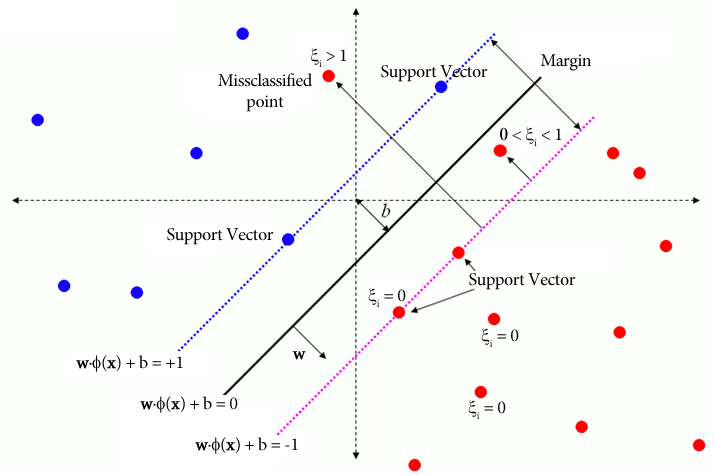
\includegraphics[keepaspectratio]{lab_2-8_files/image.png}}
\caption{image.png}
\end{figure}

    \begin{quote}
\(\textbf{Support Vector Machine (SVM)}\)
\end{quote}

    Support Vector Machine (SVM) is a supervised machine learning algorithm
used for classification and regression tasks. It tries to find the best
boundary known as hyperplane that separates different classes in the
data. It is useful when you want to do binary classification like spam
vs.~not spam or cat vs.~dog.

    SVM basically finds the boundary between different data classes and
while finding tried to find the thickest possible boundary.

    Depending on How data inside boundary area is treated SVM can eb
classified into 2 types

    \begin{enumerate}
\def\labelenumi{\arabic{enumi}.}
\tightlist
\item
  Hard margin
\item
  Soft margin
\end{enumerate}

    \begin{figure}
\centering
\pandocbounded{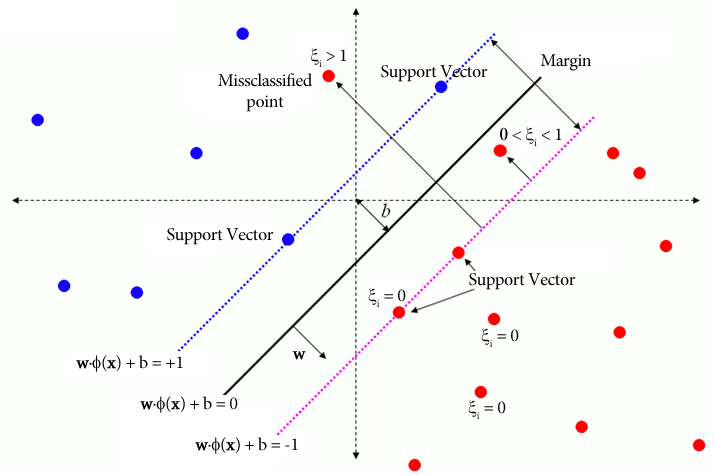
\includegraphics[keepaspectratio]{lab_2-8_files/image.png}}
\caption{image.png}
\end{figure}

    The above 2 graphs shows 2 different scenarios

    \begin{enumerate}
\def\labelenumi{\arabic{enumi}.}
\tightlist
\item
  for Hard Margin we are going to focus on the graph on left
\item
  for Soft Margin we are going to focus on the graph on the right
\end{enumerate}

    \begin{enumerate}
\def\labelenumi{\arabic{enumi}.}
\tightlist
\item
  The Dotted lines are Support vectors
\item
  The central lines are Separating hyperplane
\item
  \(M\) is th the margin
\end{enumerate}

    Central Separating Hyperplane equation =
\(\vec{W} \cdot \vec{X} + b = 0\)

    \(\color{blue}{\bullet}\) Support Vector =
\(\vec{W} \cdot \vec{X} + b = 1\)

    \(\color{red}{\blacktriangle}\) Support Vector =
\(\vec{W} \cdot \vec{X} + b = -1\)

    \(M = \frac{2}{||\vec{w}||}\) where
\(||\vec{w}|| = \sqrt{W_1^2 + W_2^2}\) for dataset with n features
\(||\vec{w}|| = \sqrt{W_1^2 + W_2^2 + ....... + W_n^2}\)

    \(\textbf{Hard Margin}\)

    For Hard Margin =\textgreater{} Algorithm:

    \(MAX \frac{2}{||\vec{W}||}=>MIN||\vec{W}||\)

    for Hard margin no data can be in the margin region

    so, based on above we can say they:

    \(y^{(i)}(\vec W \cdot \vec X) \ge 1,\; y^{(i)} \in \{-1,1\} ==>
\begin{cases}
\vec{W}\cdot\vec{X} \ge 1, & y^{(i)} = 1 \\
\vec{W}\cdot\vec{X} \le -1, & y^{(i)} = -1
\end{cases}\)

    \(\textbf{Soft Margin}\)

    for real life data soft margin is more suited as in real life data then
will be overlap in between classes which can be seen from the graph on
the right

    to consider the the data in out side its support vector slack variable
is introduced which is denoted as \(\xi\) which can be explained through
the image below

    \begin{figure}
\centering
\pandocbounded{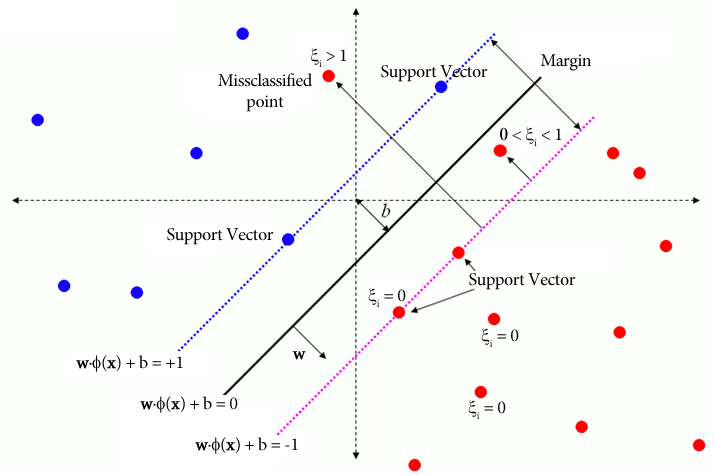
\includegraphics[keepaspectratio]{lab_2-8_files/image.png}}
\caption{image.png}
\end{figure}

    so based on the above te new constrains are as following

    \(y^{(i)}(\vec W \cdot \vec X) \ge 1 - \xi^{(i)} ==>
\begin{cases}
\vec{W}\cdot\vec{X} \ge 1 => & \xi^{(i)} = 0 \\
\vec{W}\cdot\vec{X} \le -1 => & \xi^{(i)} = 1 - Y^{(i)}(\vec{W} \cdot \vec{X} + b)
\end{cases}\)

    from the above we can get the equation to find the value of slack
variable for any \(ith\) training example which is as following

    \(\xi^{(i)} = MAX(0,1 - Y^{(i)}(\vec{W} \cdot \vec{X} + b))\)

    For Soft Margin =\textgreater{} Algorithm:

    \(MIN||\vec{w}||\) And all \(\xi^{(i)}\)

    =\textgreater{}
\(MIN_{\vec{W},b} \frac{1}{2} ||\vec{W}||^2 + C \sum_{i = 1}^{m} \xi^{(i)}\)

    for the above equation 1. we are squaring the margin of the weights
vector for gradient decent 2. The Constant C controls how much impact
the slack variable has over entire equation.

    expanding \(\xi\) in the above minimization equation

    =\textgreater{}
\(MIN_{\vec{W},b} \frac{1}{2} ||\vec{W}||^2 + C \sum_{i = 1}^{m} (1 - Y^{(i)}(\vec{W} \cdot \vec{X} + b))\)
this is main cost function

    from the above equation
\(\sum_{i = 1}^{m} (1 - Y^{(i)}(\vec{W} \cdot \vec{X} + b))\) is called
hinge loss

    \(\textbf{Hinge loss}\) =\textgreater{} if a point in data set needs
slack then it's going to have a loss and if the point does not need any
slack then the loss is zero for that point.

    \begin{quote}
\(\textbf{Naïve  Bayes}\)
\end{quote}

    The Naïve Bayes classifier is probabilistic classifier based on applying
Bayes theory with strong(naive) independent assumptions between the
features.

    Bayes equation =\textgreater{}
\(P(A|B) = \frac{P(B|A) \cdot P(A)}{P(B)}\)

    Bayes theorm states that the probability of an event A from happening
given B can be calculated by probability of B given A times probability
of A divided by probability of B

    \begin{enumerate}
\def\labelenumi{\arabic{enumi}.}
\tightlist
\item
  P(A\textbar B): Posterior Probability -- The probability of hypothesis
  A being true given that evidence B has occurred.
\item
  P(B\textbar A): Likelihood -- The probability of observing evidence B
  given that hypothesis A is true.
\item
  P(A): Prior Probability -- The initial probability of hypothesis A
  before seeing any evidence.
\item
  P(B): Marginal Likelihood (or Evidence) -- The total probability of
  observing the evidence B.
\end{enumerate}

    In our case =\textgreater{} \(P(y|X) = \frac{P(X|y) \cdot P(y)}{P(X)}\)

    where the y are the class label and X is the feature set vector

    In Naïve Bayes we assume that the features are mutually independent

    so the new equation after the assumption is as following

    \(P(y|X) = \frac{P(x_1|y) \cdot P(x_2|y) \cdot P(x_3|y) \cdot ........... P(x_n|y) \cdot P(y)}{P(X)}\)

    for the above equation \(P(y|X)\) is called posterior

    for the above equation since the denominator is independent of y and
constant for each X so we can Write the equation as following

    \(P(y|X) = P(x_1|y) \cdot P(x_2|y) \cdot P(x_3|y) \cdot ........... P(x_n|y) \cdot P(y)\)

    now to determine the class we need to select the one with highest
posterior probability so the new equation becomes

    \(\hat{y} = argmax_yP(y) \cdot P(x_1|y) \cdot P(x_2|y) \cdot P(x_3|y) \cdot ........... P(x_n|y)\)

    =\textgreater{}
\(\hat{y} = argmax_yP(y) \cdot \prod_{i = 1}^{n} P(x^i|y)\)

    \begin{quote}
\(\textbf{Data handling and TD-IDF implementation}\)
\end{quote}

    \begin{tcolorbox}[breakable, size=fbox, boxrule=1pt, pad at break*=1mm,colback=cellbackground, colframe=cellborder]
\prompt{In}{incolor}{7}{\boxspacing}
\begin{Verbatim}[commandchars=\\\{\}]
\PY{n}{path} \PY{o}{=} \PY{n}{path} \PY{o}{+} \PY{l+s+s2}{\PYZdq{}}\PY{l+s+s2}{/train.csv}\PY{l+s+s2}{\PYZdq{}}
\PY{n}{data} \PY{o}{=} \PY{n}{pd}\PY{o}{.}\PY{n}{read\PYZus{}csv}\PY{p}{(}\PY{n}{path}\PY{p}{,} \PY{n}{encoding}\PY{o}{=}\PY{l+s+s1}{\PYZsq{}}\PY{l+s+s1}{latin1}\PY{l+s+s1}{\PYZsq{}}\PY{p}{)}
\PY{n}{df} \PY{o}{=} \PY{n}{pd}\PY{o}{.}\PY{n}{DataFrame}\PY{p}{(}\PY{n}{data}\PY{p}{)}
\end{Verbatim}
\end{tcolorbox}

    \begin{tcolorbox}[breakable, size=fbox, boxrule=1pt, pad at break*=1mm,colback=cellbackground, colframe=cellborder]
\prompt{In}{incolor}{8}{\boxspacing}
\begin{Verbatim}[commandchars=\\\{\}]
\PY{n}{sentiment\PYZus{}map} \PY{o}{=} \PY{p}{\PYZob{}}
    \PY{l+s+s1}{\PYZsq{}}\PY{l+s+s1}{negative}\PY{l+s+s1}{\PYZsq{}}\PY{p}{:} \PY{l+m+mi}{0}\PY{p}{,}
    \PY{l+s+s1}{\PYZsq{}}\PY{l+s+s1}{neutral}\PY{l+s+s1}{\PYZsq{}}\PY{p}{:} \PY{l+m+mi}{1}\PY{p}{,}
    \PY{l+s+s1}{\PYZsq{}}\PY{l+s+s1}{positive}\PY{l+s+s1}{\PYZsq{}}\PY{p}{:} \PY{l+m+mi}{2}
\PY{p}{\PYZcb{}}

\PY{n}{df}\PY{p}{[}\PY{l+s+s1}{\PYZsq{}}\PY{l+s+s1}{sentiment\PYZus{}label}\PY{l+s+s1}{\PYZsq{}}\PY{p}{]} \PY{o}{=} \PY{n}{df}\PY{p}{[}\PY{l+s+s1}{\PYZsq{}}\PY{l+s+s1}{sentiment}\PY{l+s+s1}{\PYZsq{}}\PY{p}{]}\PY{o}{.}\PY{n}{map}\PY{p}{(}\PY{n}{sentiment\PYZus{}map}\PY{p}{)}
\end{Verbatim}
\end{tcolorbox}

    \begin{tcolorbox}[breakable, size=fbox, boxrule=1pt, pad at break*=1mm,colback=cellbackground, colframe=cellborder]
\prompt{In}{incolor}{9}{\boxspacing}
\begin{Verbatim}[commandchars=\\\{\}]
\PY{n}{time\PYZus{}map} \PY{o}{=} \PY{p}{\PYZob{}}
    \PY{l+s+s1}{\PYZsq{}}\PY{l+s+s1}{morning}\PY{l+s+s1}{\PYZsq{}}\PY{p}{:} \PY{p}{[}\PY{l+m+mi}{1}\PY{p}{,}\PY{l+m+mi}{0}\PY{p}{,}\PY{l+m+mi}{0}\PY{p}{]}\PY{p}{,}
    \PY{l+s+s1}{\PYZsq{}}\PY{l+s+s1}{noon}\PY{l+s+s1}{\PYZsq{}}\PY{p}{:} \PY{p}{[}\PY{l+m+mi}{0}\PY{p}{,}\PY{l+m+mi}{1}\PY{p}{,}\PY{l+m+mi}{0}\PY{p}{]}\PY{p}{,}
    \PY{l+s+s1}{\PYZsq{}}\PY{l+s+s1}{night}\PY{l+s+s1}{\PYZsq{}}\PY{p}{:} \PY{p}{[}\PY{l+m+mi}{0}\PY{p}{,}\PY{l+m+mi}{0}\PY{p}{,}\PY{l+m+mi}{1}\PY{p}{]}
\PY{p}{\PYZcb{}}

\PY{n}{df}\PY{p}{[}\PY{l+s+s1}{\PYZsq{}}\PY{l+s+s1}{time\PYZus{}label}\PY{l+s+s1}{\PYZsq{}}\PY{p}{]} \PY{o}{=} \PY{n}{df}\PY{p}{[}\PY{l+s+s1}{\PYZsq{}}\PY{l+s+s1}{Time of Tweet}\PY{l+s+s1}{\PYZsq{}}\PY{p}{]}\PY{o}{.}\PY{n}{map}\PY{p}{(}\PY{n}{time\PYZus{}map}\PY{p}{)}
\end{Verbatim}
\end{tcolorbox}

    \begin{tcolorbox}[breakable, size=fbox, boxrule=1pt, pad at break*=1mm,colback=cellbackground, colframe=cellborder]
\prompt{In}{incolor}{10}{\boxspacing}
\begin{Verbatim}[commandchars=\\\{\}]
\PY{k}{class}\PY{+w}{ }\PY{n+nc}{TfIdf}\PY{p}{:}
    \PY{k}{def}\PY{+w}{ }\PY{n+nf+fm}{\PYZus{}\PYZus{}init\PYZus{}\PYZus{}}\PY{p}{(}\PY{n+nb+bp}{self}\PY{p}{)}\PY{p}{:}
        \PY{n+nb+bp}{self}\PY{o}{.}\PY{n}{vocab} \PY{o}{=} \PY{n+nb}{set}\PY{p}{(}\PY{p}{)}
        \PY{n+nb+bp}{self}\PY{o}{.}\PY{n}{df\PYZus{}count} \PY{o}{=} \PY{p}{\PYZob{}}\PY{p}{\PYZcb{}}
        \PY{n+nb+bp}{self}\PY{o}{.}\PY{n}{idf} \PY{o}{=} \PY{p}{\PYZob{}}\PY{p}{\PYZcb{}}
        \PY{n+nb+bp}{self}\PY{o}{.}\PY{n}{N} \PY{o}{=} \PY{l+m+mi}{0}
    
    \PY{k}{def}\PY{+w}{ }\PY{n+nf}{tokenize}\PY{p}{(}\PY{n+nb+bp}{self}\PY{p}{,} \PY{n}{text}\PY{p}{)}\PY{p}{:}
        \PY{k}{if} \PY{o+ow}{not} \PY{n+nb}{isinstance}\PY{p}{(}\PY{n}{text}\PY{p}{,} \PY{n+nb}{str}\PY{p}{)}\PY{p}{:}
            \PY{k}{return} \PY{p}{[}\PY{p}{]}   \PY{c+c1}{\PYZsh{} ignore NaN or non\PYZhy{}string values}
        \PY{n}{cleaned\PYZus{}text} \PY{o}{=} \PY{n}{re}\PY{o}{.}\PY{n}{sub}\PY{p}{(}\PY{l+s+sa}{r}\PY{l+s+s2}{\PYZdq{}}\PY{l+s+s2}{[\PYZca{}}\PY{l+s+s2}{\PYZbs{}}\PY{l+s+s2}{w}\PY{l+s+s2}{\PYZbs{}}\PY{l+s+s2}{s]}\PY{l+s+s2}{\PYZdq{}}\PY{p}{,} \PY{l+s+s2}{\PYZdq{}}\PY{l+s+s2}{\PYZdq{}}\PY{p}{,} \PY{n}{text}\PY{p}{)}
        \PY{k}{return} \PY{n}{cleaned\PYZus{}text}\PY{o}{.}\PY{n}{lower}\PY{p}{(}\PY{p}{)}\PY{o}{.}\PY{n}{split}\PY{p}{(}\PY{p}{)}

    \PY{k}{def}\PY{+w}{ }\PY{n+nf}{build\PYZus{}vocab}\PY{p}{(}\PY{n+nb+bp}{self}\PY{p}{,} \PY{n}{df}\PY{p}{,} \PY{n}{column}\PY{o}{=}\PY{l+s+s1}{\PYZsq{}}\PY{l+s+s1}{message}\PY{l+s+s1}{\PYZsq{}}\PY{p}{)}\PY{p}{:}
\PY{+w}{        }\PY{l+s+sd}{\PYZdq{}\PYZdq{}\PYZdq{}Build vocabulary from all documents\PYZdq{}\PYZdq{}\PYZdq{}}
        \PY{n+nb+bp}{self}\PY{o}{.}\PY{n}{vocab} \PY{o}{=} \PY{n+nb}{set}\PY{p}{(}\PY{p}{)}
        
        \PY{k}{for} \PY{n}{i} \PY{o+ow}{in} \PY{n+nb}{range}\PY{p}{(}\PY{n+nb}{len}\PY{p}{(}\PY{n}{df}\PY{p}{)}\PY{p}{)}\PY{p}{:}
            \PY{n}{tokens} \PY{o}{=} \PY{n+nb+bp}{self}\PY{o}{.}\PY{n}{tokenize}\PY{p}{(}\PY{n}{df}\PY{o}{.}\PY{n}{loc}\PY{p}{[}\PY{n}{i}\PY{p}{,} \PY{n}{column}\PY{p}{]}\PY{p}{)}
            \PY{n+nb+bp}{self}\PY{o}{.}\PY{n}{vocab} \PY{o}{=} \PY{n+nb+bp}{self}\PY{o}{.}\PY{n}{vocab}\PY{o}{.}\PY{n}{union}\PY{p}{(}\PY{n}{tokens}\PY{p}{)}
        
        \PY{k}{return} \PY{n+nb+bp}{self}\PY{o}{.}\PY{n}{vocab}
    
    \PY{k}{def}\PY{+w}{ }\PY{n+nf}{compute\PYZus{}tf}\PY{p}{(}\PY{n+nb+bp}{self}\PY{p}{,} \PY{n}{tokens}\PY{p}{)}\PY{p}{:}
\PY{+w}{        }\PY{l+s+sd}{\PYZdq{}\PYZdq{}\PYZdq{}Compute term frequency for a document\PYZdq{}\PYZdq{}\PYZdq{}}
        \PY{k}{if} \PY{o+ow}{not} \PY{n}{tokens}\PY{p}{:}
            \PY{k}{return} \PY{p}{\PYZob{}}\PY{p}{\PYZcb{}}
        \PY{n}{tf} \PY{o}{=} \PY{n}{Counter}\PY{p}{(}\PY{n}{tokens}\PY{p}{)}
        \PY{n}{total} \PY{o}{=} \PY{n+nb}{len}\PY{p}{(}\PY{n}{tokens}\PY{p}{)}
        \PY{k}{return} \PY{p}{\PYZob{}}\PY{n}{word}\PY{p}{:} \PY{n}{count} \PY{o}{/} \PY{n}{total} \PY{k}{for} \PY{n}{word}\PY{p}{,} \PY{n}{count} \PY{o+ow}{in} \PY{n}{tf}\PY{o}{.}\PY{n}{items}\PY{p}{(}\PY{p}{)}\PY{p}{\PYZcb{}}

    \PY{k}{def}\PY{+w}{ }\PY{n+nf}{compute\PYZus{}df\PYZus{}count}\PY{p}{(}\PY{n+nb+bp}{self}\PY{p}{,} \PY{n}{df}\PY{p}{,} \PY{n}{column}\PY{o}{=}\PY{l+s+s1}{\PYZsq{}}\PY{l+s+s1}{message}\PY{l+s+s1}{\PYZsq{}}\PY{p}{)}\PY{p}{:}
\PY{+w}{        }\PY{l+s+sd}{\PYZdq{}\PYZdq{}\PYZdq{}Count document frequency for each word\PYZdq{}\PYZdq{}\PYZdq{}}
        \PY{n+nb+bp}{self}\PY{o}{.}\PY{n}{df\PYZus{}count} \PY{o}{=} \PY{n+nb}{dict}\PY{o}{.}\PY{n}{fromkeys}\PY{p}{(}\PY{n+nb+bp}{self}\PY{o}{.}\PY{n}{vocab}\PY{p}{,} \PY{l+m+mi}{0}\PY{p}{)}
        \PY{n+nb+bp}{self}\PY{o}{.}\PY{n}{N} \PY{o}{=} \PY{n+nb}{len}\PY{p}{(}\PY{n}{df}\PY{p}{)}

        \PY{k}{for} \PY{n}{i} \PY{o+ow}{in} \PY{n+nb}{range}\PY{p}{(}\PY{n+nb}{len}\PY{p}{(}\PY{n}{df}\PY{p}{)}\PY{p}{)}\PY{p}{:}
            \PY{n}{text} \PY{o}{=} \PY{n}{df}\PY{o}{.}\PY{n}{loc}\PY{p}{[}\PY{n}{i}\PY{p}{,} \PY{n}{column}\PY{p}{]}
            \PY{n}{tokens} \PY{o}{=} \PY{n+nb}{set}\PY{p}{(}\PY{n+nb+bp}{self}\PY{o}{.}\PY{n}{tokenize}\PY{p}{(}\PY{n}{text}\PY{p}{)}\PY{p}{)}  \PY{c+c1}{\PYZsh{} IMPORTANT: set() to count each word once per document}
            \PY{k}{for} \PY{n}{word} \PY{o+ow}{in} \PY{n}{tokens}\PY{p}{:}
                \PY{k}{if} \PY{n}{word} \PY{o+ow}{in} \PY{n+nb+bp}{self}\PY{o}{.}\PY{n}{df\PYZus{}count}\PY{p}{:}
                    \PY{n+nb+bp}{self}\PY{o}{.}\PY{n}{df\PYZus{}count}\PY{p}{[}\PY{n}{word}\PY{p}{]} \PY{o}{+}\PY{o}{=} \PY{l+m+mi}{1}
        
        \PY{k}{return} \PY{n+nb+bp}{self}\PY{o}{.}\PY{n}{df\PYZus{}count}
    
    \PY{k}{def}\PY{+w}{ }\PY{n+nf}{compute\PYZus{}idf}\PY{p}{(}\PY{n+nb+bp}{self}\PY{p}{)}\PY{p}{:}
\PY{+w}{        }\PY{l+s+sd}{\PYZdq{}\PYZdq{}\PYZdq{}Compute IDF values for all words in vocabulary\PYZdq{}\PYZdq{}\PYZdq{}}
        \PY{n+nb+bp}{self}\PY{o}{.}\PY{n}{idf} \PY{o}{=} \PY{p}{\PYZob{}}\PY{p}{\PYZcb{}}
        \PY{k}{for} \PY{n}{word}\PY{p}{,} \PY{n}{df\PYZus{}val} \PY{o+ow}{in} \PY{n+nb+bp}{self}\PY{o}{.}\PY{n}{df\PYZus{}count}\PY{o}{.}\PY{n}{items}\PY{p}{(}\PY{p}{)}\PY{p}{:}
            \PY{n+nb+bp}{self}\PY{o}{.}\PY{n}{idf}\PY{p}{[}\PY{n}{word}\PY{p}{]} \PY{o}{=} \PY{n}{np}\PY{o}{.}\PY{n}{log}\PY{p}{(}\PY{p}{(}\PY{n+nb+bp}{self}\PY{o}{.}\PY{n}{N} \PY{o}{+} \PY{l+m+mi}{1}\PY{p}{)} \PY{o}{/} \PY{p}{(}\PY{n}{df\PYZus{}val} \PY{o}{+} \PY{l+m+mi}{1}\PY{p}{)}\PY{p}{)} \PY{o}{+} \PY{l+m+mi}{1}
        
        \PY{k}{return} \PY{n+nb+bp}{self}\PY{o}{.}\PY{n}{idf}
    
    \PY{k}{def}\PY{+w}{ }\PY{n+nf}{compute\PYZus{}tfidf}\PY{p}{(}\PY{n+nb+bp}{self}\PY{p}{,} \PY{n}{tf}\PY{p}{)}\PY{p}{:}
\PY{+w}{        }\PY{l+s+sd}{\PYZdq{}\PYZdq{}\PYZdq{}Compute TF\PYZhy{}IDF scores given TF values\PYZdq{}\PYZdq{}\PYZdq{}}
        \PY{k}{return} \PY{p}{\PYZob{}}\PY{n}{word}\PY{p}{:} \PY{n}{tf}\PY{p}{[}\PY{n}{word}\PY{p}{]} \PY{o}{*} \PY{n+nb+bp}{self}\PY{o}{.}\PY{n}{idf}\PY{o}{.}\PY{n}{get}\PY{p}{(}\PY{n}{word}\PY{p}{,} \PY{l+m+mi}{0}\PY{p}{)} \PY{k}{for} \PY{n}{word} \PY{o+ow}{in} \PY{n}{tf}\PY{p}{\PYZcb{}}

    \PY{k}{def}\PY{+w}{ }\PY{n+nf}{compute\PYZus{}text\PYZus{}tfidf}\PY{p}{(}\PY{n+nb+bp}{self}\PY{p}{,} \PY{n}{text}\PY{p}{)}\PY{p}{:}
\PY{+w}{        }\PY{l+s+sd}{\PYZdq{}\PYZdq{}\PYZdq{}Compute TF\PYZhy{}IDF for a single text document\PYZdq{}\PYZdq{}\PYZdq{}}
        \PY{n}{tokens} \PY{o}{=} \PY{n+nb+bp}{self}\PY{o}{.}\PY{n}{tokenize}\PY{p}{(}\PY{n}{text}\PY{p}{)}
        \PY{n}{tf} \PY{o}{=} \PY{n+nb+bp}{self}\PY{o}{.}\PY{n}{compute\PYZus{}tf}\PY{p}{(}\PY{n}{tokens}\PY{p}{)}
        \PY{k}{return} \PY{n+nb+bp}{self}\PY{o}{.}\PY{n}{compute\PYZus{}tfidf}\PY{p}{(}\PY{n}{tf}\PY{p}{)}
    
    \PY{k}{def}\PY{+w}{ }\PY{n+nf}{fit}\PY{p}{(}\PY{n+nb+bp}{self}\PY{p}{,} \PY{n}{df}\PY{p}{,} \PY{n}{column}\PY{o}{=}\PY{l+s+s1}{\PYZsq{}}\PY{l+s+s1}{message}\PY{l+s+s1}{\PYZsq{}}\PY{p}{)}\PY{p}{:}
\PY{+w}{        }\PY{l+s+sd}{\PYZdq{}\PYZdq{}\PYZdq{}Fit the TF\PYZhy{}IDF model on a dataframe\PYZdq{}\PYZdq{}\PYZdq{}}
        \PY{n+nb+bp}{self}\PY{o}{.}\PY{n}{build\PYZus{}vocab}\PY{p}{(}\PY{n}{df}\PY{p}{,} \PY{n}{column}\PY{p}{)}
        \PY{n+nb+bp}{self}\PY{o}{.}\PY{n}{compute\PYZus{}df\PYZus{}count}\PY{p}{(}\PY{n}{df}\PY{p}{,} \PY{n}{column}\PY{p}{)}
        \PY{n+nb+bp}{self}\PY{o}{.}\PY{n}{compute\PYZus{}idf}\PY{p}{(}\PY{p}{)}
        \PY{k}{return} \PY{n+nb+bp}{self}
    
    \PY{k}{def}\PY{+w}{ }\PY{n+nf}{transform}\PY{p}{(}\PY{n+nb+bp}{self}\PY{p}{,} \PY{n}{df}\PY{p}{,} \PY{n}{column}\PY{o}{=}\PY{l+s+s1}{\PYZsq{}}\PY{l+s+s1}{message}\PY{l+s+s1}{\PYZsq{}}\PY{p}{)}\PY{p}{:}
\PY{+w}{        }\PY{l+s+sd}{\PYZdq{}\PYZdq{}\PYZdq{}Transform documents to TF\PYZhy{}IDF vectors\PYZdq{}\PYZdq{}\PYZdq{}}
        \PY{n}{tfidf\PYZus{}scores} \PY{o}{=} \PY{p}{[}\PY{p}{]}
        \PY{k}{for} \PY{n}{i} \PY{o+ow}{in} \PY{n+nb}{range}\PY{p}{(}\PY{n+nb}{len}\PY{p}{(}\PY{n}{df}\PY{p}{)}\PY{p}{)}\PY{p}{:}
            \PY{n}{text} \PY{o}{=} \PY{n}{df}\PY{o}{.}\PY{n}{loc}\PY{p}{[}\PY{n}{i}\PY{p}{,} \PY{n}{column}\PY{p}{]}
            \PY{n}{tfidf} \PY{o}{=} \PY{n+nb+bp}{self}\PY{o}{.}\PY{n}{compute\PYZus{}text\PYZus{}tfidf}\PY{p}{(}\PY{n}{text}\PY{p}{)}
            \PY{n}{tfidf\PYZus{}scores}\PY{o}{.}\PY{n}{append}\PY{p}{(}\PY{n}{tfidf}\PY{p}{)}
        \PY{k}{return} \PY{n}{tfidf\PYZus{}scores}
    
    \PY{k}{def}\PY{+w}{ }\PY{n+nf}{fit\PYZus{}transform}\PY{p}{(}\PY{n+nb+bp}{self}\PY{p}{,} \PY{n}{df}\PY{p}{,} \PY{n}{column}\PY{o}{=}\PY{l+s+s1}{\PYZsq{}}\PY{l+s+s1}{message}\PY{l+s+s1}{\PYZsq{}}\PY{p}{)}\PY{p}{:}
\PY{+w}{        }\PY{l+s+sd}{\PYZdq{}\PYZdq{}\PYZdq{}Fit and transform in one step\PYZdq{}\PYZdq{}\PYZdq{}}
        \PY{n+nb+bp}{self}\PY{o}{.}\PY{n}{fit}\PY{p}{(}\PY{n}{df}\PY{p}{,} \PY{n}{column}\PY{p}{)}
        \PY{k}{return} \PY{n+nb+bp}{self}\PY{o}{.}\PY{n}{transform}\PY{p}{(}\PY{n}{df}\PY{p}{,} \PY{n}{column}\PY{p}{)}
\end{Verbatim}
\end{tcolorbox}

    \begin{tcolorbox}[breakable, size=fbox, boxrule=1pt, pad at break*=1mm,colback=cellbackground, colframe=cellborder]
\prompt{In}{incolor}{11}{\boxspacing}
\begin{Verbatim}[commandchars=\\\{\}]
\PY{c+c1}{\PYZsh{} Initialize the TF\PYZhy{}IDF model}
\PY{n}{tfidf\PYZus{}model} \PY{o}{=} \PY{n}{TfIdf}\PY{p}{(}\PY{p}{)}

\PY{c+c1}{\PYZsh{} Option 1: Get dictionaries first (like your original code)}
\PY{n}{df}\PY{p}{[}\PY{l+s+s1}{\PYZsq{}}\PY{l+s+s1}{text\PYZus{}tf\PYZus{}idf}\PY{l+s+s1}{\PYZsq{}}\PY{p}{]} \PY{o}{=} \PY{n}{tfidf\PYZus{}model}\PY{o}{.}\PY{n}{fit\PYZus{}transform}\PY{p}{(}\PY{n}{df}\PY{p}{,} \PY{n}{column}\PY{o}{=}\PY{l+s+s1}{\PYZsq{}}\PY{l+s+s1}{text}\PY{l+s+s1}{\PYZsq{}}\PY{p}{)}

\PY{c+c1}{\PYZsh{} Then vectorize (exactly like your original code)}
\PY{n}{vectorizer} \PY{o}{=} \PY{n}{DictVectorizer}\PY{p}{(}\PY{n}{sparse}\PY{o}{=}\PY{k+kc}{False}\PY{p}{)}
\PY{n}{X\PYZus{}all} \PY{o}{=} \PY{n}{vectorizer}\PY{o}{.}\PY{n}{fit\PYZus{}transform}\PY{p}{(}\PY{n}{df}\PY{p}{[}\PY{l+s+s1}{\PYZsq{}}\PY{l+s+s1}{text\PYZus{}tf\PYZus{}idf}\PY{l+s+s1}{\PYZsq{}}\PY{p}{]}\PY{o}{.}\PY{n}{tolist}\PY{p}{(}\PY{p}{)}\PY{p}{)}
\PY{n}{y\PYZus{}all} \PY{o}{=} \PY{n}{df}\PY{p}{[}\PY{l+s+s1}{\PYZsq{}}\PY{l+s+s1}{sentiment\PYZus{}label}\PY{l+s+s1}{\PYZsq{}}\PY{p}{]}\PY{o}{.}\PY{n}{values}
\end{Verbatim}
\end{tcolorbox}

    \begin{tcolorbox}[breakable, size=fbox, boxrule=1pt, pad at break*=1mm,colback=cellbackground, colframe=cellborder]
\prompt{In}{incolor}{12}{\boxspacing}
\begin{Verbatim}[commandchars=\\\{\}]
\PY{c+c1}{\PYZsh{} Use only a sample of your data}
\PY{n}{sample\PYZus{}size} \PY{o}{=} \PY{l+m+mi}{5000}  \PY{c+c1}{\PYZsh{} Adjust based on your PC\PYZsq{}s RAM}
\PY{n}{df\PYZus{}sample} \PY{o}{=} \PY{n}{df}\PY{o}{.}\PY{n}{sample}\PY{p}{(}\PY{n}{n}\PY{o}{=}\PY{n}{sample\PYZus{}size}\PY{p}{,} \PY{n}{random\PYZus{}state}\PY{o}{=}\PY{l+m+mi}{42}\PY{p}{)}

\PY{c+c1}{\PYZsh{} Then convert to vectors}
\PY{n}{vectorizer} \PY{o}{=} \PY{n}{DictVectorizer}\PY{p}{(}\PY{n}{sparse}\PY{o}{=}\PY{k+kc}{False}\PY{p}{)}
\PY{n}{X\PYZus{}sample} \PY{o}{=} \PY{n}{vectorizer}\PY{o}{.}\PY{n}{fit\PYZus{}transform}\PY{p}{(}\PY{n}{df\PYZus{}sample}\PY{p}{[}\PY{l+s+s1}{\PYZsq{}}\PY{l+s+s1}{text\PYZus{}tf\PYZus{}idf}\PY{l+s+s1}{\PYZsq{}}\PY{p}{]}\PY{o}{.}\PY{n}{tolist}\PY{p}{(}\PY{p}{)}\PY{p}{)}
\PY{n}{y\PYZus{}sample} \PY{o}{=} \PY{n}{df\PYZus{}sample}\PY{p}{[}\PY{l+s+s1}{\PYZsq{}}\PY{l+s+s1}{sentiment\PYZus{}label}\PY{l+s+s1}{\PYZsq{}}\PY{p}{]}\PY{o}{.}\PY{n}{values}

\PY{c+c1}{\PYZsh{} Now split \PYZhy{} this should work}
\PY{n}{X\PYZus{}train}\PY{p}{,} \PY{n}{X\PYZus{}test}\PY{p}{,} \PY{n}{y\PYZus{}train}\PY{p}{,} \PY{n}{y\PYZus{}test} \PY{o}{=} \PY{n}{train\PYZus{}test\PYZus{}split}\PY{p}{(}
    \PY{n}{X\PYZus{}sample}\PY{p}{,} \PY{n}{y\PYZus{}sample}\PY{p}{,} \PY{n}{test\PYZus{}size}\PY{o}{=}\PY{l+m+mf}{0.2}\PY{p}{,} \PY{n}{random\PYZus{}state}\PY{o}{=}\PY{l+m+mi}{42}\PY{p}{,} \PY{n}{stratify}\PY{o}{=}\PY{n}{y\PYZus{}sample}
\PY{p}{)}
\end{Verbatim}
\end{tcolorbox}

    \begin{quote}
\(\textbf{KNN Code}\)
\end{quote}

    \begin{tcolorbox}[breakable, size=fbox, boxrule=1pt, pad at break*=1mm,colback=cellbackground, colframe=cellborder]
\prompt{In}{incolor}{13}{\boxspacing}
\begin{Verbatim}[commandchars=\\\{\}]
\PY{k}{def}\PY{+w}{ }\PY{n+nf}{euclidean\PYZus{}dist}\PY{p}{(}\PY{n}{p}\PY{p}{,}\PY{n}{q}\PY{p}{)}\PY{p}{:}
    \PY{k}{return} \PY{n}{np}\PY{o}{.}\PY{n}{sqrt}\PY{p}{(}\PY{n}{np}\PY{o}{.}\PY{n}{sum}\PY{p}{(}\PY{p}{(}\PY{n}{np}\PY{o}{.}\PY{n}{array}\PY{p}{(}\PY{n}{p}\PY{p}{)} \PY{o}{\PYZhy{}} \PY{n}{np}\PY{o}{.}\PY{n}{array}\PY{p}{(}\PY{n}{q}\PY{p}{)}\PY{p}{)}\PY{o}{*}\PY{o}{*}\PY{l+m+mi}{2}\PY{p}{)}\PY{p}{)}
\end{Verbatim}
\end{tcolorbox}

    \begin{tcolorbox}[breakable, size=fbox, boxrule=1pt, pad at break*=1mm,colback=cellbackground, colframe=cellborder]
\prompt{In}{incolor}{14}{\boxspacing}
\begin{Verbatim}[commandchars=\\\{\}]
\PY{c+c1}{\PYZsh{} 4. Modify your KNN class to work with the data format}
\PY{k}{class}\PY{+w}{ }\PY{n+nc}{KNN}\PY{p}{:}
    \PY{k}{def}\PY{+w}{ }\PY{n+nf+fm}{\PYZus{}\PYZus{}init\PYZus{}\PYZus{}}\PY{p}{(}\PY{n+nb+bp}{self}\PY{p}{,} \PY{n}{k}\PY{o}{=}\PY{l+m+mi}{3}\PY{p}{)}\PY{p}{:}
        \PY{n+nb+bp}{self}\PY{o}{.}\PY{n}{k} \PY{o}{=} \PY{n}{k}
        \PY{n+nb+bp}{self}\PY{o}{.}\PY{n}{X\PYZus{}train} \PY{o}{=} \PY{k+kc}{None}
        \PY{n+nb+bp}{self}\PY{o}{.}\PY{n}{y\PYZus{}train} \PY{o}{=} \PY{k+kc}{None}
    
    \PY{k}{def}\PY{+w}{ }\PY{n+nf}{fit}\PY{p}{(}\PY{n+nb+bp}{self}\PY{p}{,} \PY{n}{X\PYZus{}train}\PY{p}{,} \PY{n}{y\PYZus{}train}\PY{p}{)}\PY{p}{:}
\PY{+w}{        }\PY{l+s+sd}{\PYZdq{}\PYZdq{}\PYZdq{}Store training data\PYZdq{}\PYZdq{}\PYZdq{}}
        \PY{n+nb+bp}{self}\PY{o}{.}\PY{n}{X\PYZus{}train} \PY{o}{=} \PY{n}{X\PYZus{}train}
        \PY{n+nb+bp}{self}\PY{o}{.}\PY{n}{y\PYZus{}train} \PY{o}{=} \PY{n}{y\PYZus{}train}
    
    \PY{k}{def}\PY{+w}{ }\PY{n+nf}{predict}\PY{p}{(}\PY{n+nb+bp}{self}\PY{p}{,} \PY{n}{X\PYZus{}test}\PY{p}{)}\PY{p}{:}
\PY{+w}{        }\PY{l+s+sd}{\PYZdq{}\PYZdq{}\PYZdq{}Predict labels for test data\PYZdq{}\PYZdq{}\PYZdq{}}
        \PY{n}{predictions} \PY{o}{=} \PY{p}{[}\PY{p}{]}
        
        \PY{k}{for} \PY{n}{test\PYZus{}point} \PY{o+ow}{in} \PY{n}{X\PYZus{}test}\PY{p}{:}
            \PY{c+c1}{\PYZsh{} Calculate distances to all training points}
            \PY{n}{distances} \PY{o}{=} \PY{p}{[}\PY{p}{]}
            \PY{k}{for} \PY{n}{i}\PY{p}{,} \PY{n}{train\PYZus{}point} \PY{o+ow}{in} \PY{n+nb}{enumerate}\PY{p}{(}\PY{n+nb+bp}{self}\PY{o}{.}\PY{n}{X\PYZus{}train}\PY{p}{)}\PY{p}{:}
                \PY{n}{distance} \PY{o}{=} \PY{n}{euclidean\PYZus{}dist}\PY{p}{(}\PY{n}{train\PYZus{}point}\PY{p}{,} \PY{n}{test\PYZus{}point}\PY{p}{)}
                \PY{n}{distances}\PY{o}{.}\PY{n}{append}\PY{p}{(}\PY{p}{(}\PY{n}{distance}\PY{p}{,} \PY{n+nb+bp}{self}\PY{o}{.}\PY{n}{y\PYZus{}train}\PY{p}{[}\PY{n}{i}\PY{p}{]}\PY{p}{)}\PY{p}{)}
            
            \PY{c+c1}{\PYZsh{} Sort by distance and get k nearest neighbors}
            \PY{n}{distances}\PY{o}{.}\PY{n}{sort}\PY{p}{(}\PY{n}{key}\PY{o}{=}\PY{k}{lambda} \PY{n}{x}\PY{p}{:} \PY{n}{x}\PY{p}{[}\PY{l+m+mi}{0}\PY{p}{]}\PY{p}{)}
            \PY{n}{k\PYZus{}nearest} \PY{o}{=} \PY{n}{distances}\PY{p}{[}\PY{p}{:}\PY{n+nb+bp}{self}\PY{o}{.}\PY{n}{k}\PY{p}{]}
            
            \PY{c+c1}{\PYZsh{} Get the most common label}
            \PY{n}{k\PYZus{}labels} \PY{o}{=} \PY{p}{[}\PY{n}{label} \PY{k}{for} \PY{n}{\PYZus{}}\PY{p}{,} \PY{n}{label} \PY{o+ow}{in} \PY{n}{k\PYZus{}nearest}\PY{p}{]}
            \PY{n}{prediction} \PY{o}{=} \PY{n}{Counter}\PY{p}{(}\PY{n}{k\PYZus{}labels}\PY{p}{)}\PY{o}{.}\PY{n}{most\PYZus{}common}\PY{p}{(}\PY{l+m+mi}{1}\PY{p}{)}\PY{p}{[}\PY{l+m+mi}{0}\PY{p}{]}\PY{p}{[}\PY{l+m+mi}{0}\PY{p}{]}
            \PY{n}{predictions}\PY{o}{.}\PY{n}{append}\PY{p}{(}\PY{n}{prediction}\PY{p}{)}
        
        \PY{k}{return} \PY{n}{np}\PY{o}{.}\PY{n}{array}\PY{p}{(}\PY{n}{predictions}\PY{p}{)}
\end{Verbatim}
\end{tcolorbox}

    \begin{tcolorbox}[breakable, size=fbox, boxrule=1pt, pad at break*=1mm,colback=cellbackground, colframe=cellborder]
\prompt{In}{incolor}{15}{\boxspacing}
\begin{Verbatim}[commandchars=\\\{\}]
\PY{n}{k} \PY{o}{=} \PY{n}{KNN}\PY{p}{(}\PY{n}{k}\PY{o}{=}\PY{l+m+mi}{5}\PY{p}{)}
\PY{n}{k}\PY{o}{.}\PY{n}{fit}\PY{p}{(}\PY{n}{X\PYZus{}train}\PY{p}{,}\PY{n}{y\PYZus{}train}\PY{p}{)}
\PY{n}{y\PYZus{}prid} \PY{o}{=} \PY{n}{k}\PY{o}{.}\PY{n}{predict}\PY{p}{(}\PY{n}{X\PYZus{}test}\PY{p}{)}
\end{Verbatim}
\end{tcolorbox}

    \begin{quote}
\(\textbf{Confusion Matrix}\)
\end{quote}

    Confusion matrix is a simple table used to measure how well a
classification model is performing. It compares the predictions made by
the model with the actual results and shows where the model was right or
wrong. This helps you understand where the model is making mistakes so
you can improve it. It breaks down the predictions into four categories

    True Positive (TP): The model correctly predicted a positive outcome i.e
the actual outcome was positive.

    True Negative (TN): The model correctly predicted a negative outcome i.e
the actual outcome was negative.

    False Positive (FP): The model incorrectly predicted a positive outcome
i.e the actual outcome was negative. It is also known as a Type I error.

    False Negative (FN): The model incorrectly predicted a negative outcome
i.e the actual outcome was positive. It is also known as a Type II
error.

    \begin{enumerate}
\def\labelenumi{\arabic{enumi}.}
\tightlist
\item
  \(\textbf{Accuracy:}\) Accuracy shows how many predictions the model
  got right out of all the predictions
\end{enumerate}

    \(Accuracy = \frac{TP + TN}{TP + TN + FP + FN}\)

    \begin{enumerate}
\def\labelenumi{\arabic{enumi}.}
\setcounter{enumi}{1}
\tightlist
\item
  \(\textbf{Precision:}\) Precision focus on the quality of the model's
  positive predictions.
\end{enumerate}

    \(Precision = \frac{TP}{TP + TN}\)

    \begin{enumerate}
\def\labelenumi{\arabic{enumi}.}
\setcounter{enumi}{2}
\tightlist
\item
  \(\textbf{Recall:}\) Recall measures how how good the model is at
  predicting positives.
\end{enumerate}

    \(Recall = \frac{TP}{TP + FN}\)

    \begin{enumerate}
\def\labelenumi{\arabic{enumi}.}
\setcounter{enumi}{3}
\tightlist
\item
  \(\textbf{F1-Score:}\) F1-score combines precision and recall into a
  single metric to balance their trade-off. It provides a better sense
  of a model's overall performance particularly for imbalanced datasets
\end{enumerate}

    F1-Score=
\(\frac{2 \times Precision \times Recall}{Precision + Recall}\)

    \begin{quote}
\(\textbf{Confusion Matrix Code}\)
\end{quote}

    \begin{tcolorbox}[breakable, size=fbox, boxrule=1pt, pad at break*=1mm,colback=cellbackground, colframe=cellborder]
\prompt{In}{incolor}{16}{\boxspacing}
\begin{Verbatim}[commandchars=\\\{\}]
\PY{k}{class}\PY{+w}{ }\PY{n+nc}{CM}\PY{p}{:}
    \PY{k}{def}\PY{+w}{ }\PY{n+nf}{accuracy}\PY{p}{(}\PY{n+nb+bp}{self}\PY{p}{,} \PY{n}{test}\PY{p}{,} \PY{n}{prid}\PY{p}{)}\PY{p}{:}
        \PY{n}{TP} \PY{o}{=} \PY{n}{TN} \PY{o}{=} \PY{l+m+mi}{0}
        \PY{k}{for} \PY{n}{i} \PY{o+ow}{in} \PY{n+nb}{range}\PY{p}{(}\PY{n+nb}{len}\PY{p}{(}\PY{n}{test}\PY{p}{)}\PY{p}{)}\PY{p}{:}
            \PY{k}{if} \PY{n}{test}\PY{p}{[}\PY{n}{i}\PY{p}{]} \PY{o}{==} \PY{l+m+mi}{1} \PY{o+ow}{and} \PY{n}{prid}\PY{p}{[}\PY{n}{i}\PY{p}{]} \PY{o}{==} \PY{l+m+mi}{1}\PY{p}{:}
                \PY{n}{TP} \PY{o}{+}\PY{o}{=} \PY{l+m+mi}{1}
            \PY{k}{elif} \PY{n}{test}\PY{p}{[}\PY{n}{i}\PY{p}{]} \PY{o}{==} \PY{l+m+mi}{0} \PY{o+ow}{and} \PY{n}{prid}\PY{p}{[}\PY{n}{i}\PY{p}{]} \PY{o}{==} \PY{l+m+mi}{0}\PY{p}{:}
                \PY{n}{TN} \PY{o}{+}\PY{o}{=} \PY{l+m+mi}{1}
        \PY{k}{return} \PY{p}{(}\PY{n}{TP} \PY{o}{+} \PY{n}{TN}\PY{p}{)} \PY{o}{/} \PY{n+nb}{len}\PY{p}{(}\PY{n}{test}\PY{p}{)}

    \PY{k}{def}\PY{+w}{ }\PY{n+nf}{precision}\PY{p}{(}\PY{n+nb+bp}{self}\PY{p}{,} \PY{n}{test}\PY{p}{,} \PY{n}{prid}\PY{p}{)}\PY{p}{:}
        \PY{n}{TP} \PY{o}{=} \PY{n}{FP} \PY{o}{=} \PY{l+m+mi}{0}
        \PY{k}{for} \PY{n}{i} \PY{o+ow}{in} \PY{n+nb}{range}\PY{p}{(}\PY{n+nb}{len}\PY{p}{(}\PY{n}{test}\PY{p}{)}\PY{p}{)}\PY{p}{:}
            \PY{k}{if} \PY{n}{test}\PY{p}{[}\PY{n}{i}\PY{p}{]} \PY{o}{==} \PY{l+m+mi}{1} \PY{o+ow}{and} \PY{n}{prid}\PY{p}{[}\PY{n}{i}\PY{p}{]} \PY{o}{==} \PY{l+m+mi}{1}\PY{p}{:}
                \PY{n}{TP} \PY{o}{+}\PY{o}{=} \PY{l+m+mi}{1}
            \PY{k}{elif} \PY{n}{test}\PY{p}{[}\PY{n}{i}\PY{p}{]} \PY{o}{==} \PY{l+m+mi}{0} \PY{o+ow}{and} \PY{n}{prid}\PY{p}{[}\PY{n}{i}\PY{p}{]} \PY{o}{==} \PY{l+m+mi}{1}\PY{p}{:}
                \PY{n}{FP} \PY{o}{+}\PY{o}{=} \PY{l+m+mi}{1}
        \PY{k}{return} \PY{n}{TP} \PY{o}{/} \PY{p}{(}\PY{n}{TP} \PY{o}{+} \PY{n}{FP}\PY{p}{)} \PY{k}{if} \PY{p}{(}\PY{n}{TP} \PY{o}{+} \PY{n}{FP}\PY{p}{)} \PY{o}{!=} \PY{l+m+mi}{0} \PY{k}{else} \PY{l+m+mi}{0}

    \PY{k}{def}\PY{+w}{ }\PY{n+nf}{recall}\PY{p}{(}\PY{n+nb+bp}{self}\PY{p}{,} \PY{n}{test}\PY{p}{,} \PY{n}{prid}\PY{p}{)}\PY{p}{:}
        \PY{n}{TP} \PY{o}{=} \PY{n}{FN} \PY{o}{=} \PY{l+m+mi}{0}
        \PY{k}{for} \PY{n}{i} \PY{o+ow}{in} \PY{n+nb}{range}\PY{p}{(}\PY{n+nb}{len}\PY{p}{(}\PY{n}{test}\PY{p}{)}\PY{p}{)}\PY{p}{:}
            \PY{k}{if} \PY{n}{test}\PY{p}{[}\PY{n}{i}\PY{p}{]} \PY{o}{==} \PY{l+m+mi}{1} \PY{o+ow}{and} \PY{n}{prid}\PY{p}{[}\PY{n}{i}\PY{p}{]} \PY{o}{==} \PY{l+m+mi}{1}\PY{p}{:}
                \PY{n}{TP} \PY{o}{+}\PY{o}{=} \PY{l+m+mi}{1}
            \PY{k}{elif} \PY{n}{test}\PY{p}{[}\PY{n}{i}\PY{p}{]} \PY{o}{==} \PY{l+m+mi}{1} \PY{o+ow}{and} \PY{n}{prid}\PY{p}{[}\PY{n}{i}\PY{p}{]} \PY{o}{==} \PY{l+m+mi}{0}\PY{p}{:}
                \PY{n}{FN} \PY{o}{+}\PY{o}{=} \PY{l+m+mi}{1}
        \PY{k}{return} \PY{n}{TP} \PY{o}{/} \PY{p}{(}\PY{n}{TP} \PY{o}{+} \PY{n}{FN}\PY{p}{)} \PY{k}{if} \PY{p}{(}\PY{n}{TP} \PY{o}{+} \PY{n}{FN}\PY{p}{)} \PY{o}{!=} \PY{l+m+mi}{0} \PY{k}{else} \PY{l+m+mi}{0}

    \PY{k}{def}\PY{+w}{ }\PY{n+nf}{f1\PYZus{}score}\PY{p}{(}\PY{n+nb+bp}{self}\PY{p}{,} \PY{n}{test}\PY{p}{,} \PY{n}{prid}\PY{p}{)}\PY{p}{:}
        \PY{n}{p} \PY{o}{=} \PY{n+nb+bp}{self}\PY{o}{.}\PY{n}{precision}\PY{p}{(}\PY{n}{test}\PY{p}{,} \PY{n}{prid}\PY{p}{)}
        \PY{n}{r} \PY{o}{=} \PY{n+nb+bp}{self}\PY{o}{.}\PY{n}{recall}\PY{p}{(}\PY{n}{test}\PY{p}{,} \PY{n}{prid}\PY{p}{)}
        \PY{k}{return} \PY{p}{(}\PY{l+m+mi}{2} \PY{o}{*} \PY{n}{p} \PY{o}{*} \PY{n}{r}\PY{p}{)} \PY{o}{/} \PY{p}{(}\PY{n}{p} \PY{o}{+} \PY{n}{r}\PY{p}{)} \PY{k}{if} \PY{p}{(}\PY{n}{p} \PY{o}{+} \PY{n}{r}\PY{p}{)} \PY{o}{!=} \PY{l+m+mi}{0} \PY{k}{else} \PY{l+m+mi}{0}
\end{Verbatim}
\end{tcolorbox}

    \begin{quote}
\(\textbf{KNN scoring}\)
\end{quote}

    \begin{tcolorbox}[breakable, size=fbox, boxrule=1pt, pad at break*=1mm,colback=cellbackground, colframe=cellborder]
\prompt{In}{incolor}{17}{\boxspacing}
\begin{Verbatim}[commandchars=\\\{\}]
\PY{n}{cm} \PY{o}{=} \PY{n}{CM}\PY{p}{(}\PY{p}{)}
\PY{n}{acc\PYZus{}knn} \PY{o}{=} \PY{n}{cm}\PY{o}{.}\PY{n}{accuracy}\PY{p}{(}\PY{n}{y\PYZus{}test}\PY{p}{,}\PY{n}{y\PYZus{}prid}\PY{p}{)}
\PY{n}{precision\PYZus{}knn} \PY{o}{=} \PY{n}{cm}\PY{o}{.}\PY{n}{precision}\PY{p}{(}\PY{n}{y\PYZus{}test}\PY{p}{,}\PY{n}{y\PYZus{}prid}\PY{p}{)}
\PY{n}{recall\PYZus{}knn} \PY{o}{=} \PY{n}{cm}\PY{o}{.}\PY{n}{recall}\PY{p}{(}\PY{n}{y\PYZus{}test}\PY{p}{,}\PY{n}{y\PYZus{}prid}\PY{p}{)}
\PY{n}{f1\PYZus{}knn} \PY{o}{=} \PY{n}{cm}\PY{o}{.}\PY{n}{f1\PYZus{}score}\PY{p}{(}\PY{n}{y\PYZus{}test}\PY{p}{,}\PY{n}{y\PYZus{}prid}\PY{p}{)}

\PY{n+nb}{print}\PY{p}{(}\PY{l+s+sa}{f}\PY{l+s+s2}{\PYZdq{}}\PY{l+s+s2}{Accuracy: }\PY{l+s+si}{\PYZob{}}\PY{n}{acc\PYZus{}knn}\PY{l+s+si}{:}\PY{l+s+s2}{.4f}\PY{l+s+si}{\PYZcb{}}\PY{l+s+s2}{\PYZdq{}}\PY{p}{)}
\PY{n+nb}{print}\PY{p}{(}\PY{l+s+sa}{f}\PY{l+s+s2}{\PYZdq{}}\PY{l+s+s2}{Precision: }\PY{l+s+si}{\PYZob{}}\PY{n}{precision\PYZus{}knn}\PY{l+s+si}{:}\PY{l+s+s2}{.4f}\PY{l+s+si}{\PYZcb{}}\PY{l+s+s2}{\PYZdq{}}\PY{p}{)}
\PY{n+nb}{print}\PY{p}{(}\PY{l+s+sa}{f}\PY{l+s+s2}{\PYZdq{}}\PY{l+s+s2}{Recall: }\PY{l+s+si}{\PYZob{}}\PY{n}{recall\PYZus{}knn}\PY{l+s+si}{:}\PY{l+s+s2}{.4f}\PY{l+s+si}{\PYZcb{}}\PY{l+s+s2}{\PYZdq{}}\PY{p}{)}
\PY{n+nb}{print}\PY{p}{(}\PY{l+s+sa}{f}\PY{l+s+s2}{\PYZdq{}}\PY{l+s+s2}{F1\PYZhy{}Score: }\PY{l+s+si}{\PYZob{}}\PY{n}{f1\PYZus{}knn}\PY{l+s+si}{:}\PY{l+s+s2}{.4f}\PY{l+s+si}{\PYZcb{}}\PY{l+s+s2}{\PYZdq{}}\PY{p}{)}
\end{Verbatim}
\end{tcolorbox}

    \begin{Verbatim}[commandchars=\\\{\}]
Accuracy: 0.3100
Precision: 0.6030
Recall: 0.6769
F1-Score: 0.6378
    \end{Verbatim}

    \begin{quote}
\(\textbf{Naïve  Bayes code and score}\)
\end{quote}

    \begin{tcolorbox}[breakable, size=fbox, boxrule=1pt, pad at break*=1mm,colback=cellbackground, colframe=cellborder]
\prompt{In}{incolor}{18}{\boxspacing}
\begin{Verbatim}[commandchars=\\\{\}]
\PY{k+kn}{from}\PY{+w}{ }\PY{n+nn}{sklearn}\PY{n+nn}{.}\PY{n+nn}{naive\PYZus{}bayes}\PY{+w}{ }\PY{k+kn}{import} \PY{n}{MultinomialNB}

\PY{c+c1}{\PYZsh{} Note: MultinomialNB requires non\PYZhy{}negative values}
\PY{c+c1}{\PYZsh{} If your TF\PYZhy{}IDF has negative values, use GaussianNB instead}
\PY{n}{nb\PYZus{}classifier} \PY{o}{=} \PY{n}{MultinomialNB}\PY{p}{(}\PY{p}{)}
\PY{n}{nb\PYZus{}classifier}\PY{o}{.}\PY{n}{fit}\PY{p}{(}\PY{n}{X\PYZus{}train}\PY{p}{,} \PY{n}{y\PYZus{}train}\PY{p}{)}
\PY{n}{y\PYZus{}pred\PYZus{}nb} \PY{o}{=} \PY{n}{nb\PYZus{}classifier}\PY{o}{.}\PY{n}{predict}\PY{p}{(}\PY{n}{X\PYZus{}test}\PY{p}{)}

\PY{n}{cm} \PY{o}{=} \PY{n}{CM}\PY{p}{(}\PY{p}{)}
\PY{n}{acc\PYZus{}nb} \PY{o}{=} \PY{n}{cm}\PY{o}{.}\PY{n}{accuracy}\PY{p}{(}\PY{n}{y\PYZus{}test}\PY{p}{,}\PY{n}{y\PYZus{}pred\PYZus{}nb}\PY{p}{)}
\PY{n}{precision\PYZus{}nb} \PY{o}{=} \PY{n}{cm}\PY{o}{.}\PY{n}{precision}\PY{p}{(}\PY{n}{y\PYZus{}test}\PY{p}{,}\PY{n}{y\PYZus{}pred\PYZus{}nb}\PY{p}{)}
\PY{n}{recall\PYZus{}nb} \PY{o}{=} \PY{n}{cm}\PY{o}{.}\PY{n}{recall}\PY{p}{(}\PY{n}{y\PYZus{}test}\PY{p}{,}\PY{n}{y\PYZus{}pred\PYZus{}nb}\PY{p}{)}
\PY{n}{f1\PYZus{}nb} \PY{o}{=} \PY{n}{cm}\PY{o}{.}\PY{n}{f1\PYZus{}score}\PY{p}{(}\PY{n}{y\PYZus{}test}\PY{p}{,}\PY{n}{y\PYZus{}pred\PYZus{}nb}\PY{p}{)}

\PY{n+nb}{print}\PY{p}{(}\PY{l+s+sa}{f}\PY{l+s+s2}{\PYZdq{}}\PY{l+s+s2}{Accuracy: }\PY{l+s+si}{\PYZob{}}\PY{n}{acc\PYZus{}nb}\PY{l+s+si}{:}\PY{l+s+s2}{.4f}\PY{l+s+si}{\PYZcb{}}\PY{l+s+s2}{\PYZdq{}}\PY{p}{)}
\PY{n+nb}{print}\PY{p}{(}\PY{l+s+sa}{f}\PY{l+s+s2}{\PYZdq{}}\PY{l+s+s2}{Precision: }\PY{l+s+si}{\PYZob{}}\PY{n}{precision\PYZus{}nb}\PY{l+s+si}{:}\PY{l+s+s2}{.4f}\PY{l+s+si}{\PYZcb{}}\PY{l+s+s2}{\PYZdq{}}\PY{p}{)}
\PY{n+nb}{print}\PY{p}{(}\PY{l+s+sa}{f}\PY{l+s+s2}{\PYZdq{}}\PY{l+s+s2}{Recall: }\PY{l+s+si}{\PYZob{}}\PY{n}{recall\PYZus{}nb}\PY{l+s+si}{:}\PY{l+s+s2}{.4f}\PY{l+s+si}{\PYZcb{}}\PY{l+s+s2}{\PYZdq{}}\PY{p}{)}
\PY{n+nb}{print}\PY{p}{(}\PY{l+s+sa}{f}\PY{l+s+s2}{\PYZdq{}}\PY{l+s+s2}{F1\PYZhy{}Score: }\PY{l+s+si}{\PYZob{}}\PY{n}{f1\PYZus{}nb}\PY{l+s+si}{:}\PY{l+s+s2}{.4f}\PY{l+s+si}{\PYZcb{}}\PY{l+s+s2}{\PYZdq{}}\PY{p}{)}
\end{Verbatim}
\end{tcolorbox}

    \begin{Verbatim}[commandchars=\\\{\}]
Accuracy: 0.3850
Precision: 0.6534
Recall: 0.7507
F1-Score: 0.6987
    \end{Verbatim}

    \begin{quote}
\(\textbf{SVM code and score}\)
\end{quote}

    \begin{tcolorbox}[breakable, size=fbox, boxrule=1pt, pad at break*=1mm,colback=cellbackground, colframe=cellborder]
\prompt{In}{incolor}{19}{\boxspacing}
\begin{Verbatim}[commandchars=\\\{\}]
\PY{k+kn}{from}\PY{+w}{ }\PY{n+nn}{sklearn}\PY{n+nn}{.}\PY{n+nn}{svm}\PY{+w}{ }\PY{k+kn}{import} \PY{n}{SVC}

\PY{n}{svm\PYZus{}classifier} \PY{o}{=} \PY{n}{SVC}\PY{p}{(}\PY{n}{kernel}\PY{o}{=}\PY{l+s+s1}{\PYZsq{}}\PY{l+s+s1}{linear}\PY{l+s+s1}{\PYZsq{}}\PY{p}{,} \PY{n}{C}\PY{o}{=}\PY{l+m+mf}{1.0}\PY{p}{,} \PY{n}{random\PYZus{}state}\PY{o}{=}\PY{l+m+mi}{42}\PY{p}{)}
\PY{n}{svm\PYZus{}classifier}\PY{o}{.}\PY{n}{fit}\PY{p}{(}\PY{n}{X\PYZus{}train}\PY{p}{,} \PY{n}{y\PYZus{}train}\PY{p}{)}
\PY{n}{y\PYZus{}pred\PYZus{}svm} \PY{o}{=} \PY{n}{svm\PYZus{}classifier}\PY{o}{.}\PY{n}{predict}\PY{p}{(}\PY{n}{X\PYZus{}test}\PY{p}{)}

\PY{n}{cm} \PY{o}{=} \PY{n}{CM}\PY{p}{(}\PY{p}{)}
\PY{n}{acc\PYZus{}svm} \PY{o}{=} \PY{n}{cm}\PY{o}{.}\PY{n}{accuracy}\PY{p}{(}\PY{n}{y\PYZus{}test}\PY{p}{,}\PY{n}{y\PYZus{}pred\PYZus{}svm}\PY{p}{)}
\PY{n}{precision\PYZus{}svm} \PY{o}{=} \PY{n}{cm}\PY{o}{.}\PY{n}{precision}\PY{p}{(}\PY{n}{y\PYZus{}test}\PY{p}{,}\PY{n}{y\PYZus{}pred\PYZus{}svm}\PY{p}{)}
\PY{n}{recall\PYZus{}svm} \PY{o}{=} \PY{n}{cm}\PY{o}{.}\PY{n}{recall}\PY{p}{(}\PY{n}{y\PYZus{}test}\PY{p}{,}\PY{n}{y\PYZus{}pred\PYZus{}svm}\PY{p}{)}
\PY{n}{f1\PYZus{}svm} \PY{o}{=} \PY{n}{cm}\PY{o}{.}\PY{n}{f1\PYZus{}score}\PY{p}{(}\PY{n}{y\PYZus{}test}\PY{p}{,}\PY{n}{y\PYZus{}pred\PYZus{}svm}\PY{p}{)}

\PY{n+nb}{print}\PY{p}{(}\PY{l+s+sa}{f}\PY{l+s+s2}{\PYZdq{}}\PY{l+s+s2}{Accuracy: }\PY{l+s+si}{\PYZob{}}\PY{n}{acc\PYZus{}svm}\PY{l+s+si}{:}\PY{l+s+s2}{.4f}\PY{l+s+si}{\PYZcb{}}\PY{l+s+s2}{\PYZdq{}}\PY{p}{)}
\PY{n+nb}{print}\PY{p}{(}\PY{l+s+sa}{f}\PY{l+s+s2}{\PYZdq{}}\PY{l+s+s2}{Precision: }\PY{l+s+si}{\PYZob{}}\PY{n}{precision\PYZus{}svm}\PY{l+s+si}{:}\PY{l+s+s2}{.4f}\PY{l+s+si}{\PYZcb{}}\PY{l+s+s2}{\PYZdq{}}\PY{p}{)}
\PY{n+nb}{print}\PY{p}{(}\PY{l+s+sa}{f}\PY{l+s+s2}{\PYZdq{}}\PY{l+s+s2}{Recall: }\PY{l+s+si}{\PYZob{}}\PY{n}{recall\PYZus{}svm}\PY{l+s+si}{:}\PY{l+s+s2}{.4f}\PY{l+s+si}{\PYZcb{}}\PY{l+s+s2}{\PYZdq{}}\PY{p}{)}
\PY{n+nb}{print}\PY{p}{(}\PY{l+s+sa}{f}\PY{l+s+s2}{\PYZdq{}}\PY{l+s+s2}{F1\PYZhy{}Score: }\PY{l+s+si}{\PYZob{}}\PY{n}{f1\PYZus{}svm}\PY{l+s+si}{:}\PY{l+s+s2}{.4f}\PY{l+s+si}{\PYZcb{}}\PY{l+s+s2}{\PYZdq{}}\PY{p}{)}
\end{Verbatim}
\end{tcolorbox}

    \begin{Verbatim}[commandchars=\\\{\}]
Accuracy: 0.3780
Precision: 0.6677
Recall: 0.6716
F1-Score: 0.6696
    \end{Verbatim}

    \begin{quote}
\(\textbf{KNN, SVM, Naïve  Bayes score comparison}\)
\end{quote}

    \begin{tcolorbox}[breakable, size=fbox, boxrule=1pt, pad at break*=1mm,colback=cellbackground, colframe=cellborder]
\prompt{In}{incolor}{20}{\boxspacing}
\begin{Verbatim}[commandchars=\\\{\}]
\PY{n+nb}{print}\PY{p}{(}\PY{l+s+s2}{\PYZdq{}}\PY{l+s+se}{\PYZbs{}n}\PY{l+s+s2}{\PYZdq{}} \PY{o}{+} \PY{l+s+s2}{\PYZdq{}}\PY{l+s+s2}{=}\PY{l+s+s2}{\PYZdq{}}\PY{o}{*}\PY{l+m+mi}{50}\PY{p}{)}
\PY{n+nb}{print}\PY{p}{(}\PY{l+s+s2}{\PYZdq{}}\PY{l+s+s2}{PERFORMANCE COMPARISON}\PY{l+s+s2}{\PYZdq{}}\PY{p}{)}
\PY{n+nb}{print}\PY{p}{(}\PY{l+s+s2}{\PYZdq{}}\PY{l+s+s2}{=}\PY{l+s+s2}{\PYZdq{}}\PY{o}{*}\PY{l+m+mi}{50}\PY{p}{)}

\PY{n}{comparison\PYZus{}df} \PY{o}{=} \PY{n}{pd}\PY{o}{.}\PY{n}{DataFrame}\PY{p}{(}\PY{p}{\PYZob{}}
    \PY{l+s+s1}{\PYZsq{}}\PY{l+s+s1}{Classifier}\PY{l+s+s1}{\PYZsq{}}\PY{p}{:} \PY{p}{[}\PY{l+s+s1}{\PYZsq{}}\PY{l+s+s1}{KNN}\PY{l+s+s1}{\PYZsq{}}\PY{p}{,} \PY{l+s+s1}{\PYZsq{}}\PY{l+s+s1}{Naive Bayes}\PY{l+s+s1}{\PYZsq{}}\PY{p}{,} \PY{l+s+s1}{\PYZsq{}}\PY{l+s+s1}{SVM}\PY{l+s+s1}{\PYZsq{}}\PY{p}{]}\PY{p}{,}
    \PY{l+s+s1}{\PYZsq{}}\PY{l+s+s1}{Accuracy}\PY{l+s+s1}{\PYZsq{}}\PY{p}{:} \PY{p}{[}\PY{n}{acc\PYZus{}knn}\PY{p}{,} \PY{n}{acc\PYZus{}nb}\PY{p}{,} \PY{n}{acc\PYZus{}svm}\PY{p}{]}\PY{p}{,}
    \PY{l+s+s1}{\PYZsq{}}\PY{l+s+s1}{Precision}\PY{l+s+s1}{\PYZsq{}}\PY{p}{:} \PY{p}{[}\PY{n}{precision\PYZus{}knn}\PY{p}{,} \PY{n}{precision\PYZus{}nb}\PY{p}{,} \PY{n}{precision\PYZus{}svm}\PY{p}{]}\PY{p}{,}
    \PY{l+s+s1}{\PYZsq{}}\PY{l+s+s1}{Recall}\PY{l+s+s1}{\PYZsq{}}\PY{p}{:} \PY{p}{[}\PY{n}{recall\PYZus{}knn}\PY{p}{,} \PY{n}{recall\PYZus{}nb}\PY{p}{,} \PY{n}{recall\PYZus{}svm}\PY{p}{]}\PY{p}{,}
    \PY{l+s+s1}{\PYZsq{}}\PY{l+s+s1}{F1\PYZhy{}Score}\PY{l+s+s1}{\PYZsq{}}\PY{p}{:} \PY{p}{[}\PY{n}{f1\PYZus{}knn}\PY{p}{,} \PY{n}{f1\PYZus{}nb}\PY{p}{,} \PY{n}{f1\PYZus{}svm}\PY{p}{]}
\PY{p}{\PYZcb{}}\PY{p}{)}

\PY{n+nb}{print}\PY{p}{(}\PY{n}{comparison\PYZus{}df}\PY{o}{.}\PY{n}{to\PYZus{}string}\PY{p}{(}\PY{n}{index}\PY{o}{=}\PY{k+kc}{False}\PY{p}{)}\PY{p}{)}

\PY{c+c1}{\PYZsh{} Find best classifier}
\PY{n}{best\PYZus{}idx} \PY{o}{=} \PY{n}{comparison\PYZus{}df}\PY{p}{[}\PY{l+s+s1}{\PYZsq{}}\PY{l+s+s1}{Accuracy}\PY{l+s+s1}{\PYZsq{}}\PY{p}{]}\PY{o}{.}\PY{n}{idxmax}\PY{p}{(}\PY{p}{)}
\PY{n}{best\PYZus{}classifier} \PY{o}{=} \PY{n}{comparison\PYZus{}df}\PY{o}{.}\PY{n}{loc}\PY{p}{[}\PY{n}{best\PYZus{}idx}\PY{p}{,} \PY{l+s+s1}{\PYZsq{}}\PY{l+s+s1}{Classifier}\PY{l+s+s1}{\PYZsq{}}\PY{p}{]}
\PY{n}{best\PYZus{}accuracy} \PY{o}{=} \PY{n}{comparison\PYZus{}df}\PY{o}{.}\PY{n}{loc}\PY{p}{[}\PY{n}{best\PYZus{}idx}\PY{p}{,} \PY{l+s+s1}{\PYZsq{}}\PY{l+s+s1}{Accuracy}\PY{l+s+s1}{\PYZsq{}}\PY{p}{]}
\PY{n+nb}{print}\PY{p}{(}\PY{l+s+sa}{f}\PY{l+s+s2}{\PYZdq{}}\PY{l+s+se}{\PYZbs{}n}\PY{l+s+s2}{Best Classifier: }\PY{l+s+si}{\PYZob{}}\PY{n}{best\PYZus{}classifier}\PY{l+s+si}{\PYZcb{}}\PY{l+s+s2}{ with Accuracy: }\PY{l+s+si}{\PYZob{}}\PY{n}{best\PYZus{}accuracy}\PY{l+s+si}{:}\PY{l+s+s2}{.4f}\PY{l+s+si}{\PYZcb{}}\PY{l+s+s2}{\PYZdq{}}\PY{p}{)}
\end{Verbatim}
\end{tcolorbox}

    \begin{Verbatim}[commandchars=\\\{\}]

==================================================
PERFORMANCE COMPARISON
==================================================
 Classifier  Accuracy  Precision   Recall  F1-Score
        KNN     0.310   0.603030 0.676871  0.637821
Naive Bayes     0.385   0.653367 0.750716  0.698667
        SVM     0.378   0.667656 0.671642  0.669643

Best Classifier: Naive Bayes with Accuracy: 0.3850
    \end{Verbatim}

    \begin{quote}
\(\textbf{Score Visualization}\)
\end{quote}

    \begin{tcolorbox}[breakable, size=fbox, boxrule=1pt, pad at break*=1mm,colback=cellbackground, colframe=cellborder]
\prompt{In}{incolor}{22}{\boxspacing}
\begin{Verbatim}[commandchars=\\\{\}]
\PY{c+c1}{\PYZsh{} Plot 1: Accuracy Comparison}
\PY{n}{plt}\PY{o}{.}\PY{n}{figure}\PY{p}{(}\PY{n}{figsize}\PY{o}{=}\PY{p}{(}\PY{l+m+mi}{10}\PY{p}{,} \PY{l+m+mi}{6}\PY{p}{)}\PY{p}{)}
\PY{n}{plt}\PY{o}{.}\PY{n}{bar}\PY{p}{(}\PY{n}{comparison\PYZus{}df}\PY{p}{[}\PY{l+s+s1}{\PYZsq{}}\PY{l+s+s1}{Classifier}\PY{l+s+s1}{\PYZsq{}}\PY{p}{]}\PY{p}{,} \PY{n}{comparison\PYZus{}df}\PY{p}{[}\PY{l+s+s1}{\PYZsq{}}\PY{l+s+s1}{Accuracy}\PY{l+s+s1}{\PYZsq{}}\PY{p}{]}\PY{p}{,} 
        \PY{n}{color}\PY{o}{=}\PY{p}{[}\PY{l+s+s1}{\PYZsq{}}\PY{l+s+s1}{blue}\PY{l+s+s1}{\PYZsq{}}\PY{p}{,} \PY{l+s+s1}{\PYZsq{}}\PY{l+s+s1}{green}\PY{l+s+s1}{\PYZsq{}}\PY{p}{,} \PY{l+s+s1}{\PYZsq{}}\PY{l+s+s1}{red}\PY{l+s+s1}{\PYZsq{}}\PY{p}{]}\PY{p}{,} \PY{n}{alpha}\PY{o}{=}\PY{l+m+mf}{0.7}\PY{p}{)}
\PY{n}{plt}\PY{o}{.}\PY{n}{xlabel}\PY{p}{(}\PY{l+s+s1}{\PYZsq{}}\PY{l+s+s1}{Classifier}\PY{l+s+s1}{\PYZsq{}}\PY{p}{,} \PY{n}{fontsize}\PY{o}{=}\PY{l+m+mi}{12}\PY{p}{)}
\PY{n}{plt}\PY{o}{.}\PY{n}{ylabel}\PY{p}{(}\PY{l+s+s1}{\PYZsq{}}\PY{l+s+s1}{Accuracy}\PY{l+s+s1}{\PYZsq{}}\PY{p}{,} \PY{n}{fontsize}\PY{o}{=}\PY{l+m+mi}{12}\PY{p}{)}
\PY{n}{plt}\PY{o}{.}\PY{n}{title}\PY{p}{(}\PY{l+s+s1}{\PYZsq{}}\PY{l+s+s1}{Accuracy Comparison of Classifiers}\PY{l+s+s1}{\PYZsq{}}\PY{p}{,} \PY{n}{fontsize}\PY{o}{=}\PY{l+m+mi}{14}\PY{p}{,} \PY{n}{fontweight}\PY{o}{=}\PY{l+s+s1}{\PYZsq{}}\PY{l+s+s1}{bold}\PY{l+s+s1}{\PYZsq{}}\PY{p}{)}
\PY{n}{plt}\PY{o}{.}\PY{n}{ylim}\PY{p}{(}\PY{p}{[}\PY{l+m+mi}{0}\PY{p}{,} \PY{l+m+mi}{1}\PY{p}{]}\PY{p}{)}
\PY{k}{for} \PY{n}{i}\PY{p}{,} \PY{n}{v} \PY{o+ow}{in} \PY{n+nb}{enumerate}\PY{p}{(}\PY{n}{comparison\PYZus{}df}\PY{p}{[}\PY{l+s+s1}{\PYZsq{}}\PY{l+s+s1}{Accuracy}\PY{l+s+s1}{\PYZsq{}}\PY{p}{]}\PY{p}{)}\PY{p}{:}
    \PY{n}{plt}\PY{o}{.}\PY{n}{text}\PY{p}{(}\PY{n}{i}\PY{p}{,} \PY{n}{v} \PY{o}{+} \PY{l+m+mf}{0.02}\PY{p}{,} \PY{l+s+sa}{f}\PY{l+s+s1}{\PYZsq{}}\PY{l+s+si}{\PYZob{}}\PY{n}{v}\PY{l+s+si}{:}\PY{l+s+s1}{.4f}\PY{l+s+si}{\PYZcb{}}\PY{l+s+s1}{\PYZsq{}}\PY{p}{,} \PY{n}{ha}\PY{o}{=}\PY{l+s+s1}{\PYZsq{}}\PY{l+s+s1}{center}\PY{l+s+s1}{\PYZsq{}}\PY{p}{,} \PY{n}{fontweight}\PY{o}{=}\PY{l+s+s1}{\PYZsq{}}\PY{l+s+s1}{bold}\PY{l+s+s1}{\PYZsq{}}\PY{p}{)}
\PY{n}{plt}\PY{o}{.}\PY{n}{grid}\PY{p}{(}\PY{n}{axis}\PY{o}{=}\PY{l+s+s1}{\PYZsq{}}\PY{l+s+s1}{y}\PY{l+s+s1}{\PYZsq{}}\PY{p}{,} \PY{n}{alpha}\PY{o}{=}\PY{l+m+mf}{0.3}\PY{p}{)}
\PY{n}{plt}\PY{o}{.}\PY{n}{tight\PYZus{}layout}\PY{p}{(}\PY{p}{)}
\PY{n}{plt}\PY{o}{.}\PY{n}{show}\PY{p}{(}\PY{p}{)}

\PY{c+c1}{\PYZsh{} Plot 2: All Metrics Comparison}
\PY{n}{fig}\PY{p}{,} \PY{n}{ax} \PY{o}{=} \PY{n}{plt}\PY{o}{.}\PY{n}{subplots}\PY{p}{(}\PY{n}{figsize}\PY{o}{=}\PY{p}{(}\PY{l+m+mi}{12}\PY{p}{,} \PY{l+m+mi}{6}\PY{p}{)}\PY{p}{)}
\PY{n}{x} \PY{o}{=} \PY{n}{np}\PY{o}{.}\PY{n}{arange}\PY{p}{(}\PY{n+nb}{len}\PY{p}{(}\PY{n}{comparison\PYZus{}df}\PY{p}{[}\PY{l+s+s1}{\PYZsq{}}\PY{l+s+s1}{Classifier}\PY{l+s+s1}{\PYZsq{}}\PY{p}{]}\PY{p}{)}\PY{p}{)}
\PY{n}{width} \PY{o}{=} \PY{l+m+mf}{0.2}

\PY{n}{bars1} \PY{o}{=} \PY{n}{ax}\PY{o}{.}\PY{n}{bar}\PY{p}{(}\PY{n}{x} \PY{o}{\PYZhy{}} \PY{l+m+mf}{1.5}\PY{o}{*}\PY{n}{width}\PY{p}{,} \PY{n}{comparison\PYZus{}df}\PY{p}{[}\PY{l+s+s1}{\PYZsq{}}\PY{l+s+s1}{Accuracy}\PY{l+s+s1}{\PYZsq{}}\PY{p}{]}\PY{p}{,} \PY{n}{width}\PY{p}{,} \PY{n}{label}\PY{o}{=}\PY{l+s+s1}{\PYZsq{}}\PY{l+s+s1}{Accuracy}\PY{l+s+s1}{\PYZsq{}}\PY{p}{,} \PY{n}{alpha}\PY{o}{=}\PY{l+m+mf}{0.8}\PY{p}{)}
\PY{n}{bars2} \PY{o}{=} \PY{n}{ax}\PY{o}{.}\PY{n}{bar}\PY{p}{(}\PY{n}{x} \PY{o}{\PYZhy{}} \PY{l+m+mf}{0.5}\PY{o}{*}\PY{n}{width}\PY{p}{,} \PY{n}{comparison\PYZus{}df}\PY{p}{[}\PY{l+s+s1}{\PYZsq{}}\PY{l+s+s1}{Precision}\PY{l+s+s1}{\PYZsq{}}\PY{p}{]}\PY{p}{,} \PY{n}{width}\PY{p}{,} \PY{n}{label}\PY{o}{=}\PY{l+s+s1}{\PYZsq{}}\PY{l+s+s1}{Precision}\PY{l+s+s1}{\PYZsq{}}\PY{p}{,} \PY{n}{alpha}\PY{o}{=}\PY{l+m+mf}{0.8}\PY{p}{)}
\PY{n}{bars3} \PY{o}{=} \PY{n}{ax}\PY{o}{.}\PY{n}{bar}\PY{p}{(}\PY{n}{x} \PY{o}{+} \PY{l+m+mf}{0.5}\PY{o}{*}\PY{n}{width}\PY{p}{,} \PY{n}{comparison\PYZus{}df}\PY{p}{[}\PY{l+s+s1}{\PYZsq{}}\PY{l+s+s1}{Recall}\PY{l+s+s1}{\PYZsq{}}\PY{p}{]}\PY{p}{,} \PY{n}{width}\PY{p}{,} \PY{n}{label}\PY{o}{=}\PY{l+s+s1}{\PYZsq{}}\PY{l+s+s1}{Recall}\PY{l+s+s1}{\PYZsq{}}\PY{p}{,} \PY{n}{alpha}\PY{o}{=}\PY{l+m+mf}{0.8}\PY{p}{)}
\PY{n}{bars4} \PY{o}{=} \PY{n}{ax}\PY{o}{.}\PY{n}{bar}\PY{p}{(}\PY{n}{x} \PY{o}{+} \PY{l+m+mf}{1.5}\PY{o}{*}\PY{n}{width}\PY{p}{,} \PY{n}{comparison\PYZus{}df}\PY{p}{[}\PY{l+s+s1}{\PYZsq{}}\PY{l+s+s1}{F1\PYZhy{}Score}\PY{l+s+s1}{\PYZsq{}}\PY{p}{]}\PY{p}{,} \PY{n}{width}\PY{p}{,} \PY{n}{label}\PY{o}{=}\PY{l+s+s1}{\PYZsq{}}\PY{l+s+s1}{F1\PYZhy{}Score}\PY{l+s+s1}{\PYZsq{}}\PY{p}{,} \PY{n}{alpha}\PY{o}{=}\PY{l+m+mf}{0.8}\PY{p}{)}

\PY{n}{ax}\PY{o}{.}\PY{n}{set\PYZus{}xlabel}\PY{p}{(}\PY{l+s+s1}{\PYZsq{}}\PY{l+s+s1}{Classifier}\PY{l+s+s1}{\PYZsq{}}\PY{p}{,} \PY{n}{fontsize}\PY{o}{=}\PY{l+m+mi}{12}\PY{p}{)}
\PY{n}{ax}\PY{o}{.}\PY{n}{set\PYZus{}ylabel}\PY{p}{(}\PY{l+s+s1}{\PYZsq{}}\PY{l+s+s1}{Score}\PY{l+s+s1}{\PYZsq{}}\PY{p}{,} \PY{n}{fontsize}\PY{o}{=}\PY{l+m+mi}{12}\PY{p}{)}
\PY{n}{ax}\PY{o}{.}\PY{n}{set\PYZus{}title}\PY{p}{(}\PY{l+s+s1}{\PYZsq{}}\PY{l+s+s1}{Performance Metrics Comparison}\PY{l+s+s1}{\PYZsq{}}\PY{p}{,} \PY{n}{fontsize}\PY{o}{=}\PY{l+m+mi}{14}\PY{p}{,} \PY{n}{fontweight}\PY{o}{=}\PY{l+s+s1}{\PYZsq{}}\PY{l+s+s1}{bold}\PY{l+s+s1}{\PYZsq{}}\PY{p}{)}
\PY{n}{ax}\PY{o}{.}\PY{n}{set\PYZus{}xticks}\PY{p}{(}\PY{n}{x}\PY{p}{)}
\PY{n}{ax}\PY{o}{.}\PY{n}{set\PYZus{}xticklabels}\PY{p}{(}\PY{n}{comparison\PYZus{}df}\PY{p}{[}\PY{l+s+s1}{\PYZsq{}}\PY{l+s+s1}{Classifier}\PY{l+s+s1}{\PYZsq{}}\PY{p}{]}\PY{p}{)}
\PY{n}{ax}\PY{o}{.}\PY{n}{legend}\PY{p}{(}\PY{p}{)}
\PY{n}{ax}\PY{o}{.}\PY{n}{grid}\PY{p}{(}\PY{n}{axis}\PY{o}{=}\PY{l+s+s1}{\PYZsq{}}\PY{l+s+s1}{y}\PY{l+s+s1}{\PYZsq{}}\PY{p}{,} \PY{n}{alpha}\PY{o}{=}\PY{l+m+mf}{0.3}\PY{p}{)}
\PY{n}{ax}\PY{o}{.}\PY{n}{set\PYZus{}ylim}\PY{p}{(}\PY{p}{[}\PY{l+m+mi}{0}\PY{p}{,} \PY{l+m+mi}{1}\PY{p}{]}\PY{p}{)}
\PY{n}{plt}\PY{o}{.}\PY{n}{tight\PYZus{}layout}\PY{p}{(}\PY{p}{)}
\PY{n}{plt}\PY{o}{.}\PY{n}{show}\PY{p}{(}\PY{p}{)}

\PY{c+c1}{\PYZsh{} Plot 3: Confusion Matrices}
\PY{n}{fig}\PY{p}{,} \PY{n}{axes} \PY{o}{=} \PY{n}{plt}\PY{o}{.}\PY{n}{subplots}\PY{p}{(}\PY{l+m+mi}{1}\PY{p}{,} \PY{l+m+mi}{3}\PY{p}{,} \PY{n}{figsize}\PY{o}{=}\PY{p}{(}\PY{l+m+mi}{18}\PY{p}{,} \PY{l+m+mi}{5}\PY{p}{)}\PY{p}{)}

\PY{c+c1}{\PYZsh{} KNN Confusion Matrix}
\PY{n}{cm\PYZus{}knn} \PY{o}{=} \PY{n}{confusion\PYZus{}matrix}\PY{p}{(}\PY{n}{y\PYZus{}test}\PY{p}{,} \PY{n}{y\PYZus{}prid}\PY{p}{)}
\PY{n}{sns}\PY{o}{.}\PY{n}{heatmap}\PY{p}{(}\PY{n}{cm\PYZus{}knn}\PY{p}{,} \PY{n}{annot}\PY{o}{=}\PY{k+kc}{True}\PY{p}{,} \PY{n}{fmt}\PY{o}{=}\PY{l+s+s1}{\PYZsq{}}\PY{l+s+s1}{d}\PY{l+s+s1}{\PYZsq{}}\PY{p}{,} \PY{n}{cmap}\PY{o}{=}\PY{l+s+s1}{\PYZsq{}}\PY{l+s+s1}{Blues}\PY{l+s+s1}{\PYZsq{}}\PY{p}{,} \PY{n}{ax}\PY{o}{=}\PY{n}{axes}\PY{p}{[}\PY{l+m+mi}{0}\PY{p}{]}\PY{p}{,}
            \PY{n}{xticklabels}\PY{o}{=}\PY{p}{[}\PY{l+s+s1}{\PYZsq{}}\PY{l+s+s1}{Negative}\PY{l+s+s1}{\PYZsq{}}\PY{p}{,} \PY{l+s+s1}{\PYZsq{}}\PY{l+s+s1}{Neutral}\PY{l+s+s1}{\PYZsq{}}\PY{p}{,} \PY{l+s+s1}{\PYZsq{}}\PY{l+s+s1}{Positive}\PY{l+s+s1}{\PYZsq{}}\PY{p}{]}\PY{p}{,}
            \PY{n}{yticklabels}\PY{o}{=}\PY{p}{[}\PY{l+s+s1}{\PYZsq{}}\PY{l+s+s1}{Negative}\PY{l+s+s1}{\PYZsq{}}\PY{p}{,} \PY{l+s+s1}{\PYZsq{}}\PY{l+s+s1}{Neutral}\PY{l+s+s1}{\PYZsq{}}\PY{p}{,} \PY{l+s+s1}{\PYZsq{}}\PY{l+s+s1}{Positive}\PY{l+s+s1}{\PYZsq{}}\PY{p}{]}\PY{p}{)}
\PY{n}{axes}\PY{p}{[}\PY{l+m+mi}{0}\PY{p}{]}\PY{o}{.}\PY{n}{set\PYZus{}title}\PY{p}{(}\PY{l+s+sa}{f}\PY{l+s+s1}{\PYZsq{}}\PY{l+s+s1}{KNN}\PY{l+s+se}{\PYZbs{}n}\PY{l+s+s1}{Accuracy: }\PY{l+s+si}{\PYZob{}}\PY{n}{acc\PYZus{}knn}\PY{l+s+si}{:}\PY{l+s+s1}{.4f}\PY{l+s+si}{\PYZcb{}}\PY{l+s+s1}{\PYZsq{}}\PY{p}{,} \PY{n}{fontweight}\PY{o}{=}\PY{l+s+s1}{\PYZsq{}}\PY{l+s+s1}{bold}\PY{l+s+s1}{\PYZsq{}}\PY{p}{)}
\PY{n}{axes}\PY{p}{[}\PY{l+m+mi}{0}\PY{p}{]}\PY{o}{.}\PY{n}{set\PYZus{}ylabel}\PY{p}{(}\PY{l+s+s1}{\PYZsq{}}\PY{l+s+s1}{True Label}\PY{l+s+s1}{\PYZsq{}}\PY{p}{)}
\PY{n}{axes}\PY{p}{[}\PY{l+m+mi}{0}\PY{p}{]}\PY{o}{.}\PY{n}{set\PYZus{}xlabel}\PY{p}{(}\PY{l+s+s1}{\PYZsq{}}\PY{l+s+s1}{Predicted Label}\PY{l+s+s1}{\PYZsq{}}\PY{p}{)}

\PY{c+c1}{\PYZsh{} Naive Bayes Confusion Matrix}
\PY{n}{cm\PYZus{}nb} \PY{o}{=} \PY{n}{confusion\PYZus{}matrix}\PY{p}{(}\PY{n}{y\PYZus{}test}\PY{p}{,} \PY{n}{y\PYZus{}pred\PYZus{}nb}\PY{p}{)}
\PY{n}{sns}\PY{o}{.}\PY{n}{heatmap}\PY{p}{(}\PY{n}{cm\PYZus{}nb}\PY{p}{,} \PY{n}{annot}\PY{o}{=}\PY{k+kc}{True}\PY{p}{,} \PY{n}{fmt}\PY{o}{=}\PY{l+s+s1}{\PYZsq{}}\PY{l+s+s1}{d}\PY{l+s+s1}{\PYZsq{}}\PY{p}{,} \PY{n}{cmap}\PY{o}{=}\PY{l+s+s1}{\PYZsq{}}\PY{l+s+s1}{Greens}\PY{l+s+s1}{\PYZsq{}}\PY{p}{,} \PY{n}{ax}\PY{o}{=}\PY{n}{axes}\PY{p}{[}\PY{l+m+mi}{1}\PY{p}{]}\PY{p}{,}
            \PY{n}{xticklabels}\PY{o}{=}\PY{p}{[}\PY{l+s+s1}{\PYZsq{}}\PY{l+s+s1}{Negative}\PY{l+s+s1}{\PYZsq{}}\PY{p}{,} \PY{l+s+s1}{\PYZsq{}}\PY{l+s+s1}{Neutral}\PY{l+s+s1}{\PYZsq{}}\PY{p}{,} \PY{l+s+s1}{\PYZsq{}}\PY{l+s+s1}{Positive}\PY{l+s+s1}{\PYZsq{}}\PY{p}{]}\PY{p}{,}
            \PY{n}{yticklabels}\PY{o}{=}\PY{p}{[}\PY{l+s+s1}{\PYZsq{}}\PY{l+s+s1}{Negative}\PY{l+s+s1}{\PYZsq{}}\PY{p}{,} \PY{l+s+s1}{\PYZsq{}}\PY{l+s+s1}{Neutral}\PY{l+s+s1}{\PYZsq{}}\PY{p}{,} \PY{l+s+s1}{\PYZsq{}}\PY{l+s+s1}{Positive}\PY{l+s+s1}{\PYZsq{}}\PY{p}{]}\PY{p}{)}
\PY{n}{axes}\PY{p}{[}\PY{l+m+mi}{1}\PY{p}{]}\PY{o}{.}\PY{n}{set\PYZus{}title}\PY{p}{(}\PY{l+s+sa}{f}\PY{l+s+s1}{\PYZsq{}}\PY{l+s+s1}{Naive Bayes}\PY{l+s+se}{\PYZbs{}n}\PY{l+s+s1}{Accuracy: }\PY{l+s+si}{\PYZob{}}\PY{n}{acc\PYZus{}nb}\PY{l+s+si}{:}\PY{l+s+s1}{.4f}\PY{l+s+si}{\PYZcb{}}\PY{l+s+s1}{\PYZsq{}}\PY{p}{,} \PY{n}{fontweight}\PY{o}{=}\PY{l+s+s1}{\PYZsq{}}\PY{l+s+s1}{bold}\PY{l+s+s1}{\PYZsq{}}\PY{p}{)}
\PY{n}{axes}\PY{p}{[}\PY{l+m+mi}{1}\PY{p}{]}\PY{o}{.}\PY{n}{set\PYZus{}ylabel}\PY{p}{(}\PY{l+s+s1}{\PYZsq{}}\PY{l+s+s1}{True Label}\PY{l+s+s1}{\PYZsq{}}\PY{p}{)}
\PY{n}{axes}\PY{p}{[}\PY{l+m+mi}{1}\PY{p}{]}\PY{o}{.}\PY{n}{set\PYZus{}xlabel}\PY{p}{(}\PY{l+s+s1}{\PYZsq{}}\PY{l+s+s1}{Predicted Label}\PY{l+s+s1}{\PYZsq{}}\PY{p}{)}

\PY{c+c1}{\PYZsh{} SVM Confusion Matrix}
\PY{n}{cm\PYZus{}svm} \PY{o}{=} \PY{n}{confusion\PYZus{}matrix}\PY{p}{(}\PY{n}{y\PYZus{}test}\PY{p}{,} \PY{n}{y\PYZus{}pred\PYZus{}svm}\PY{p}{)}
\PY{n}{sns}\PY{o}{.}\PY{n}{heatmap}\PY{p}{(}\PY{n}{cm\PYZus{}svm}\PY{p}{,} \PY{n}{annot}\PY{o}{=}\PY{k+kc}{True}\PY{p}{,} \PY{n}{fmt}\PY{o}{=}\PY{l+s+s1}{\PYZsq{}}\PY{l+s+s1}{d}\PY{l+s+s1}{\PYZsq{}}\PY{p}{,} \PY{n}{cmap}\PY{o}{=}\PY{l+s+s1}{\PYZsq{}}\PY{l+s+s1}{Reds}\PY{l+s+s1}{\PYZsq{}}\PY{p}{,} \PY{n}{ax}\PY{o}{=}\PY{n}{axes}\PY{p}{[}\PY{l+m+mi}{2}\PY{p}{]}\PY{p}{,}
            \PY{n}{xticklabels}\PY{o}{=}\PY{p}{[}\PY{l+s+s1}{\PYZsq{}}\PY{l+s+s1}{Negative}\PY{l+s+s1}{\PYZsq{}}\PY{p}{,} \PY{l+s+s1}{\PYZsq{}}\PY{l+s+s1}{Neutral}\PY{l+s+s1}{\PYZsq{}}\PY{p}{,} \PY{l+s+s1}{\PYZsq{}}\PY{l+s+s1}{Positive}\PY{l+s+s1}{\PYZsq{}}\PY{p}{]}\PY{p}{,}
            \PY{n}{yticklabels}\PY{o}{=}\PY{p}{[}\PY{l+s+s1}{\PYZsq{}}\PY{l+s+s1}{Negative}\PY{l+s+s1}{\PYZsq{}}\PY{p}{,} \PY{l+s+s1}{\PYZsq{}}\PY{l+s+s1}{Neutral}\PY{l+s+s1}{\PYZsq{}}\PY{p}{,} \PY{l+s+s1}{\PYZsq{}}\PY{l+s+s1}{Positive}\PY{l+s+s1}{\PYZsq{}}\PY{p}{]}\PY{p}{)}
\PY{n}{axes}\PY{p}{[}\PY{l+m+mi}{2}\PY{p}{]}\PY{o}{.}\PY{n}{set\PYZus{}title}\PY{p}{(}\PY{l+s+sa}{f}\PY{l+s+s1}{\PYZsq{}}\PY{l+s+s1}{SVM}\PY{l+s+se}{\PYZbs{}n}\PY{l+s+s1}{Accuracy: }\PY{l+s+si}{\PYZob{}}\PY{n}{acc\PYZus{}svm}\PY{l+s+si}{:}\PY{l+s+s1}{.4f}\PY{l+s+si}{\PYZcb{}}\PY{l+s+s1}{\PYZsq{}}\PY{p}{,} \PY{n}{fontweight}\PY{o}{=}\PY{l+s+s1}{\PYZsq{}}\PY{l+s+s1}{bold}\PY{l+s+s1}{\PYZsq{}}\PY{p}{)}
\PY{n}{axes}\PY{p}{[}\PY{l+m+mi}{2}\PY{p}{]}\PY{o}{.}\PY{n}{set\PYZus{}ylabel}\PY{p}{(}\PY{l+s+s1}{\PYZsq{}}\PY{l+s+s1}{True Label}\PY{l+s+s1}{\PYZsq{}}\PY{p}{)}
\PY{n}{axes}\PY{p}{[}\PY{l+m+mi}{2}\PY{p}{]}\PY{o}{.}\PY{n}{set\PYZus{}xlabel}\PY{p}{(}\PY{l+s+s1}{\PYZsq{}}\PY{l+s+s1}{Predicted Label}\PY{l+s+s1}{\PYZsq{}}\PY{p}{)}

\PY{n}{plt}\PY{o}{.}\PY{n}{tight\PYZus{}layout}\PY{p}{(}\PY{p}{)}
\PY{n}{plt}\PY{o}{.}\PY{n}{show}\PY{p}{(}\PY{p}{)}

\PY{c+c1}{\PYZsh{} ============================================}
\PY{c+c1}{\PYZsh{} 6. TEST WITH NEW EXAMPLES (Optional)}
\PY{c+c1}{\PYZsh{} ============================================}
\PY{n+nb}{print}\PY{p}{(}\PY{l+s+s2}{\PYZdq{}}\PY{l+s+se}{\PYZbs{}n}\PY{l+s+s2}{\PYZdq{}} \PY{o}{+} \PY{l+s+s2}{\PYZdq{}}\PY{l+s+s2}{=}\PY{l+s+s2}{\PYZdq{}}\PY{o}{*}\PY{l+m+mi}{50}\PY{p}{)}
\PY{n+nb}{print}\PY{p}{(}\PY{l+s+s2}{\PYZdq{}}\PY{l+s+s2}{TESTING WITH NEW EXAMPLES}\PY{l+s+s2}{\PYZdq{}}\PY{p}{)}
\PY{n+nb}{print}\PY{p}{(}\PY{l+s+s2}{\PYZdq{}}\PY{l+s+s2}{=}\PY{l+s+s2}{\PYZdq{}}\PY{o}{*}\PY{l+m+mi}{50}\PY{p}{)}

\PY{c+c1}{\PYZsh{} Example reviews}
\PY{n}{test\PYZus{}reviews} \PY{o}{=} \PY{p}{[}
    \PY{l+s+s2}{\PYZdq{}}\PY{l+s+s2}{This product is absolutely amazing! I love it!}\PY{l+s+s2}{\PYZdq{}}\PY{p}{,}
    \PY{l+s+s2}{\PYZdq{}}\PY{l+s+s2}{Terrible experience, waste of money.}\PY{l+s+s2}{\PYZdq{}}\PY{p}{,}
    \PY{l+s+s2}{\PYZdq{}}\PY{l+s+s2}{It}\PY{l+s+s2}{\PYZsq{}}\PY{l+s+s2}{s okay, nothing special.}\PY{l+s+s2}{\PYZdq{}}
\PY{p}{]}

\PY{n}{tfidf\PYZus{}model} \PY{o}{=} \PY{n}{TfIdf}\PY{p}{(}\PY{p}{)}

\PY{k}{for} \PY{n}{review} \PY{o+ow}{in} \PY{n}{test\PYZus{}reviews}\PY{p}{:}
    \PY{c+c1}{\PYZsh{} Convert to TF\PYZhy{}IDF}
    \PY{n}{review\PYZus{}tfidf} \PY{o}{=} \PY{n}{tfidf\PYZus{}model}\PY{o}{.}\PY{n}{compute\PYZus{}text\PYZus{}tfidf}\PY{p}{(}\PY{n}{review}\PY{p}{)}
    \PY{n}{review\PYZus{}vector} \PY{o}{=} \PY{n}{vectorizer}\PY{o}{.}\PY{n}{transform}\PY{p}{(}\PY{p}{[}\PY{n}{review\PYZus{}tfidf}\PY{p}{]}\PY{p}{)}
    
    \PY{c+c1}{\PYZsh{} Predict with all classifiers}
    \PY{n}{pred\PYZus{}knn} \PY{o}{=} \PY{n}{k}\PY{o}{.}\PY{n}{predict}\PY{p}{(}\PY{n}{review\PYZus{}vector}\PY{p}{)}\PY{p}{[}\PY{l+m+mi}{0}\PY{p}{]}
    \PY{n}{pred\PYZus{}nb} \PY{o}{=} \PY{n}{nb\PYZus{}classifier}\PY{o}{.}\PY{n}{predict}\PY{p}{(}\PY{n}{review\PYZus{}vector}\PY{p}{)}\PY{p}{[}\PY{l+m+mi}{0}\PY{p}{]}
    \PY{n}{pred\PYZus{}svm} \PY{o}{=} \PY{n}{svm\PYZus{}classifier}\PY{o}{.}\PY{n}{predict}\PY{p}{(}\PY{n}{review\PYZus{}vector}\PY{p}{)}\PY{p}{[}\PY{l+m+mi}{0}\PY{p}{]}
    
    \PY{n}{sentiment\PYZus{}names} \PY{o}{=} \PY{p}{\PYZob{}}\PY{l+m+mi}{0}\PY{p}{:} \PY{l+s+s1}{\PYZsq{}}\PY{l+s+s1}{Negative}\PY{l+s+s1}{\PYZsq{}}\PY{p}{,} \PY{l+m+mi}{1}\PY{p}{:} \PY{l+s+s1}{\PYZsq{}}\PY{l+s+s1}{Neutral}\PY{l+s+s1}{\PYZsq{}}\PY{p}{,} \PY{l+m+mi}{2}\PY{p}{:} \PY{l+s+s1}{\PYZsq{}}\PY{l+s+s1}{Positive}\PY{l+s+s1}{\PYZsq{}}\PY{p}{\PYZcb{}}
    
    \PY{n+nb}{print}\PY{p}{(}\PY{l+s+sa}{f}\PY{l+s+s2}{\PYZdq{}}\PY{l+s+se}{\PYZbs{}n}\PY{l+s+s2}{Review: }\PY{l+s+s2}{\PYZsq{}}\PY{l+s+si}{\PYZob{}}\PY{n}{review}\PY{l+s+si}{\PYZcb{}}\PY{l+s+s2}{\PYZsq{}}\PY{l+s+s2}{\PYZdq{}}\PY{p}{)}
    \PY{n+nb}{print}\PY{p}{(}\PY{l+s+sa}{f}\PY{l+s+s2}{\PYZdq{}}\PY{l+s+s2}{  KNN Prediction: }\PY{l+s+si}{\PYZob{}}\PY{n}{sentiment\PYZus{}names}\PY{p}{[}\PY{n}{pred\PYZus{}knn}\PY{p}{]}\PY{l+s+si}{\PYZcb{}}\PY{l+s+s2}{\PYZdq{}}\PY{p}{)}
    \PY{n+nb}{print}\PY{p}{(}\PY{l+s+sa}{f}\PY{l+s+s2}{\PYZdq{}}\PY{l+s+s2}{  Naive Bayes Prediction: }\PY{l+s+si}{\PYZob{}}\PY{n}{sentiment\PYZus{}names}\PY{p}{[}\PY{n}{pred\PYZus{}nb}\PY{p}{]}\PY{l+s+si}{\PYZcb{}}\PY{l+s+s2}{\PYZdq{}}\PY{p}{)}
    \PY{n+nb}{print}\PY{p}{(}\PY{l+s+sa}{f}\PY{l+s+s2}{\PYZdq{}}\PY{l+s+s2}{  SVM Prediction: }\PY{l+s+si}{\PYZob{}}\PY{n}{sentiment\PYZus{}names}\PY{p}{[}\PY{n}{pred\PYZus{}svm}\PY{p}{]}\PY{l+s+si}{\PYZcb{}}\PY{l+s+s2}{\PYZdq{}}\PY{p}{)}
\end{Verbatim}
\end{tcolorbox}

    \begin{center}
    \adjustimage{max size={0.9\linewidth}{0.9\paperheight}}{lab_2-8_files/lab_2-8_98_0.png}
    \end{center}
    { \hspace*{\fill} \\}
    
    \begin{center}
    \adjustimage{max size={0.9\linewidth}{0.9\paperheight}}{lab_2-8_files/lab_2-8_98_1.png}
    \end{center}
    { \hspace*{\fill} \\}
    
    \begin{center}
    \adjustimage{max size={0.9\linewidth}{0.9\paperheight}}{lab_2-8_files/lab_2-8_98_2.png}
    \end{center}
    { \hspace*{\fill} \\}
    
    \begin{Verbatim}[commandchars=\\\{\}]

==================================================
TESTING WITH NEW EXAMPLES
==================================================

Review: 'This product is absolutely amazing! I love it!'
  KNN Prediction: Neutral
  Naive Bayes Prediction: Neutral
  SVM Prediction: Neutral

Review: 'Terrible experience, waste of money.'
  KNN Prediction: Neutral
  Naive Bayes Prediction: Neutral
  SVM Prediction: Neutral

Review: 'It's okay, nothing special.'
  KNN Prediction: Neutral
  Naive Bayes Prediction: Neutral
  SVM Prediction: Neutral
    \end{Verbatim}


    % Add a bibliography block to the postdoc
    
    
    
\end{document}
